%!TEX root = ../thesis.tex
% ******************************* Thesis Appendix B ********************************

\chapter{Additional information to Chapter 3} \label{appendix:CTtrain}
This Appendix contains supplementary figures for Chapter~\ref{chap:CT_method}.


\section{Supplementary Figures}
\label{sectionB1.1}

\begin{figure}[ht!]
    \centering    
    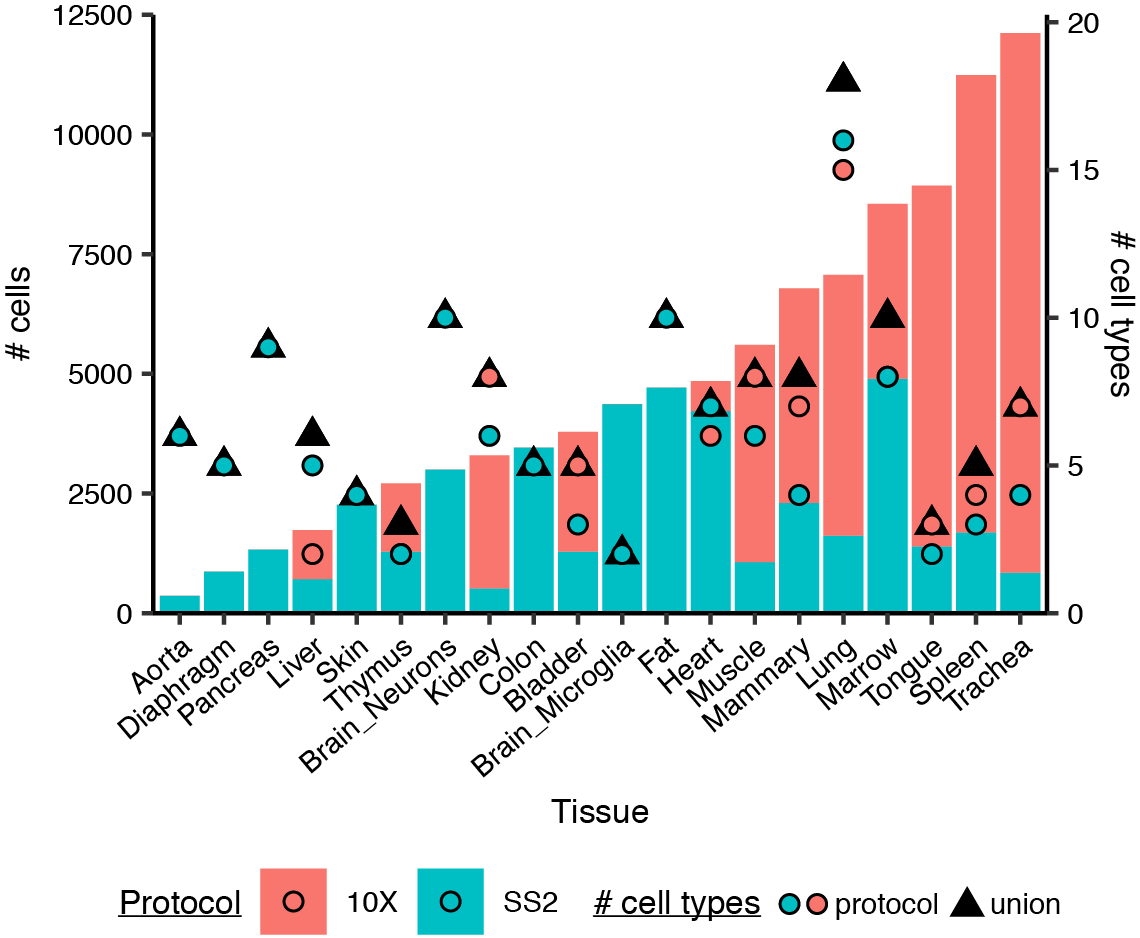
\includegraphics[scale=1.1]{Appendix2/Figs/countsCTCells_TabulaMuris.png} % change word in curlies to change figure
    \caption[Cell numbers in the \textit{Tabula Muris} dataset]{\textbf{Cell numbers in the \textit{Tabula Muris} dataset} \newline Bars show number of cells (left y axis) collected from different tissues (x axis), split by scRNA-seq protocol (colour). Points show the number of cell types (right y axis) identified by protocol (coloured circles) or their union (triangle). 10X - Chromium (10X Genomics) protocol; SS2 - Smart-seq2 protocol.}
    \label{fig:appB_tmcounts}
\end{figure}


\begin{figure}[pht!] 
\centering    
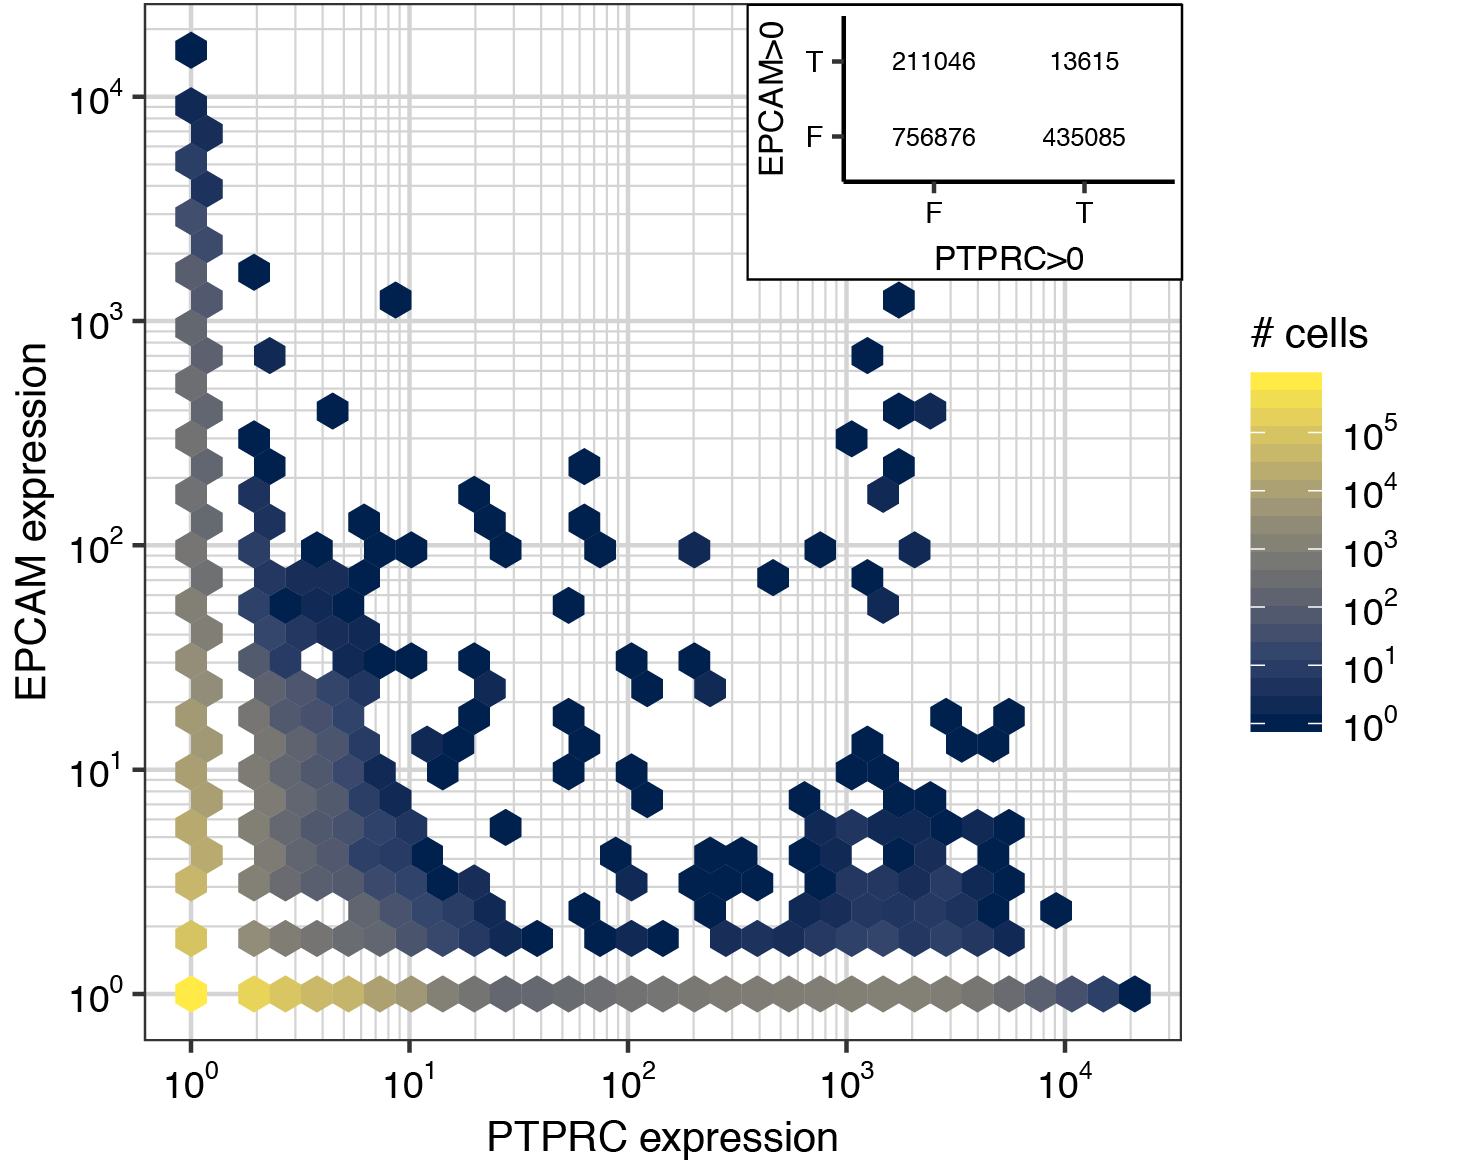
\includegraphics[scale=0.81]{Appendix2/Figs/PTPRC_EPCAM_human.png} % change word in curlies to change figure
\caption[Expression of \textit{PTPRC} and \textit{EPCAM} in human data collection]{\textbf{Expression of \textit{PTPRC} and \textit{EPCAM} in human data collection (Related to Figure~\ref{fig:chap3_humancells})}\newline2D-binned plot of single-cell expression of \textit{PTPRC} (encoding for the CD45 receptor, an immune cell marker), and \textit{EPCAM} (an epithelial cell marker). Inset table (top right) shows the number of cell expressing (T) or not (F) each of the genes. Cells expressing both genes are likely doublets or affected by ambient RNA in droplet-based experiments.}
\label{fig:appB_ptprc}
\end{figure}


\begin{figure}[ht!] 
\centering    
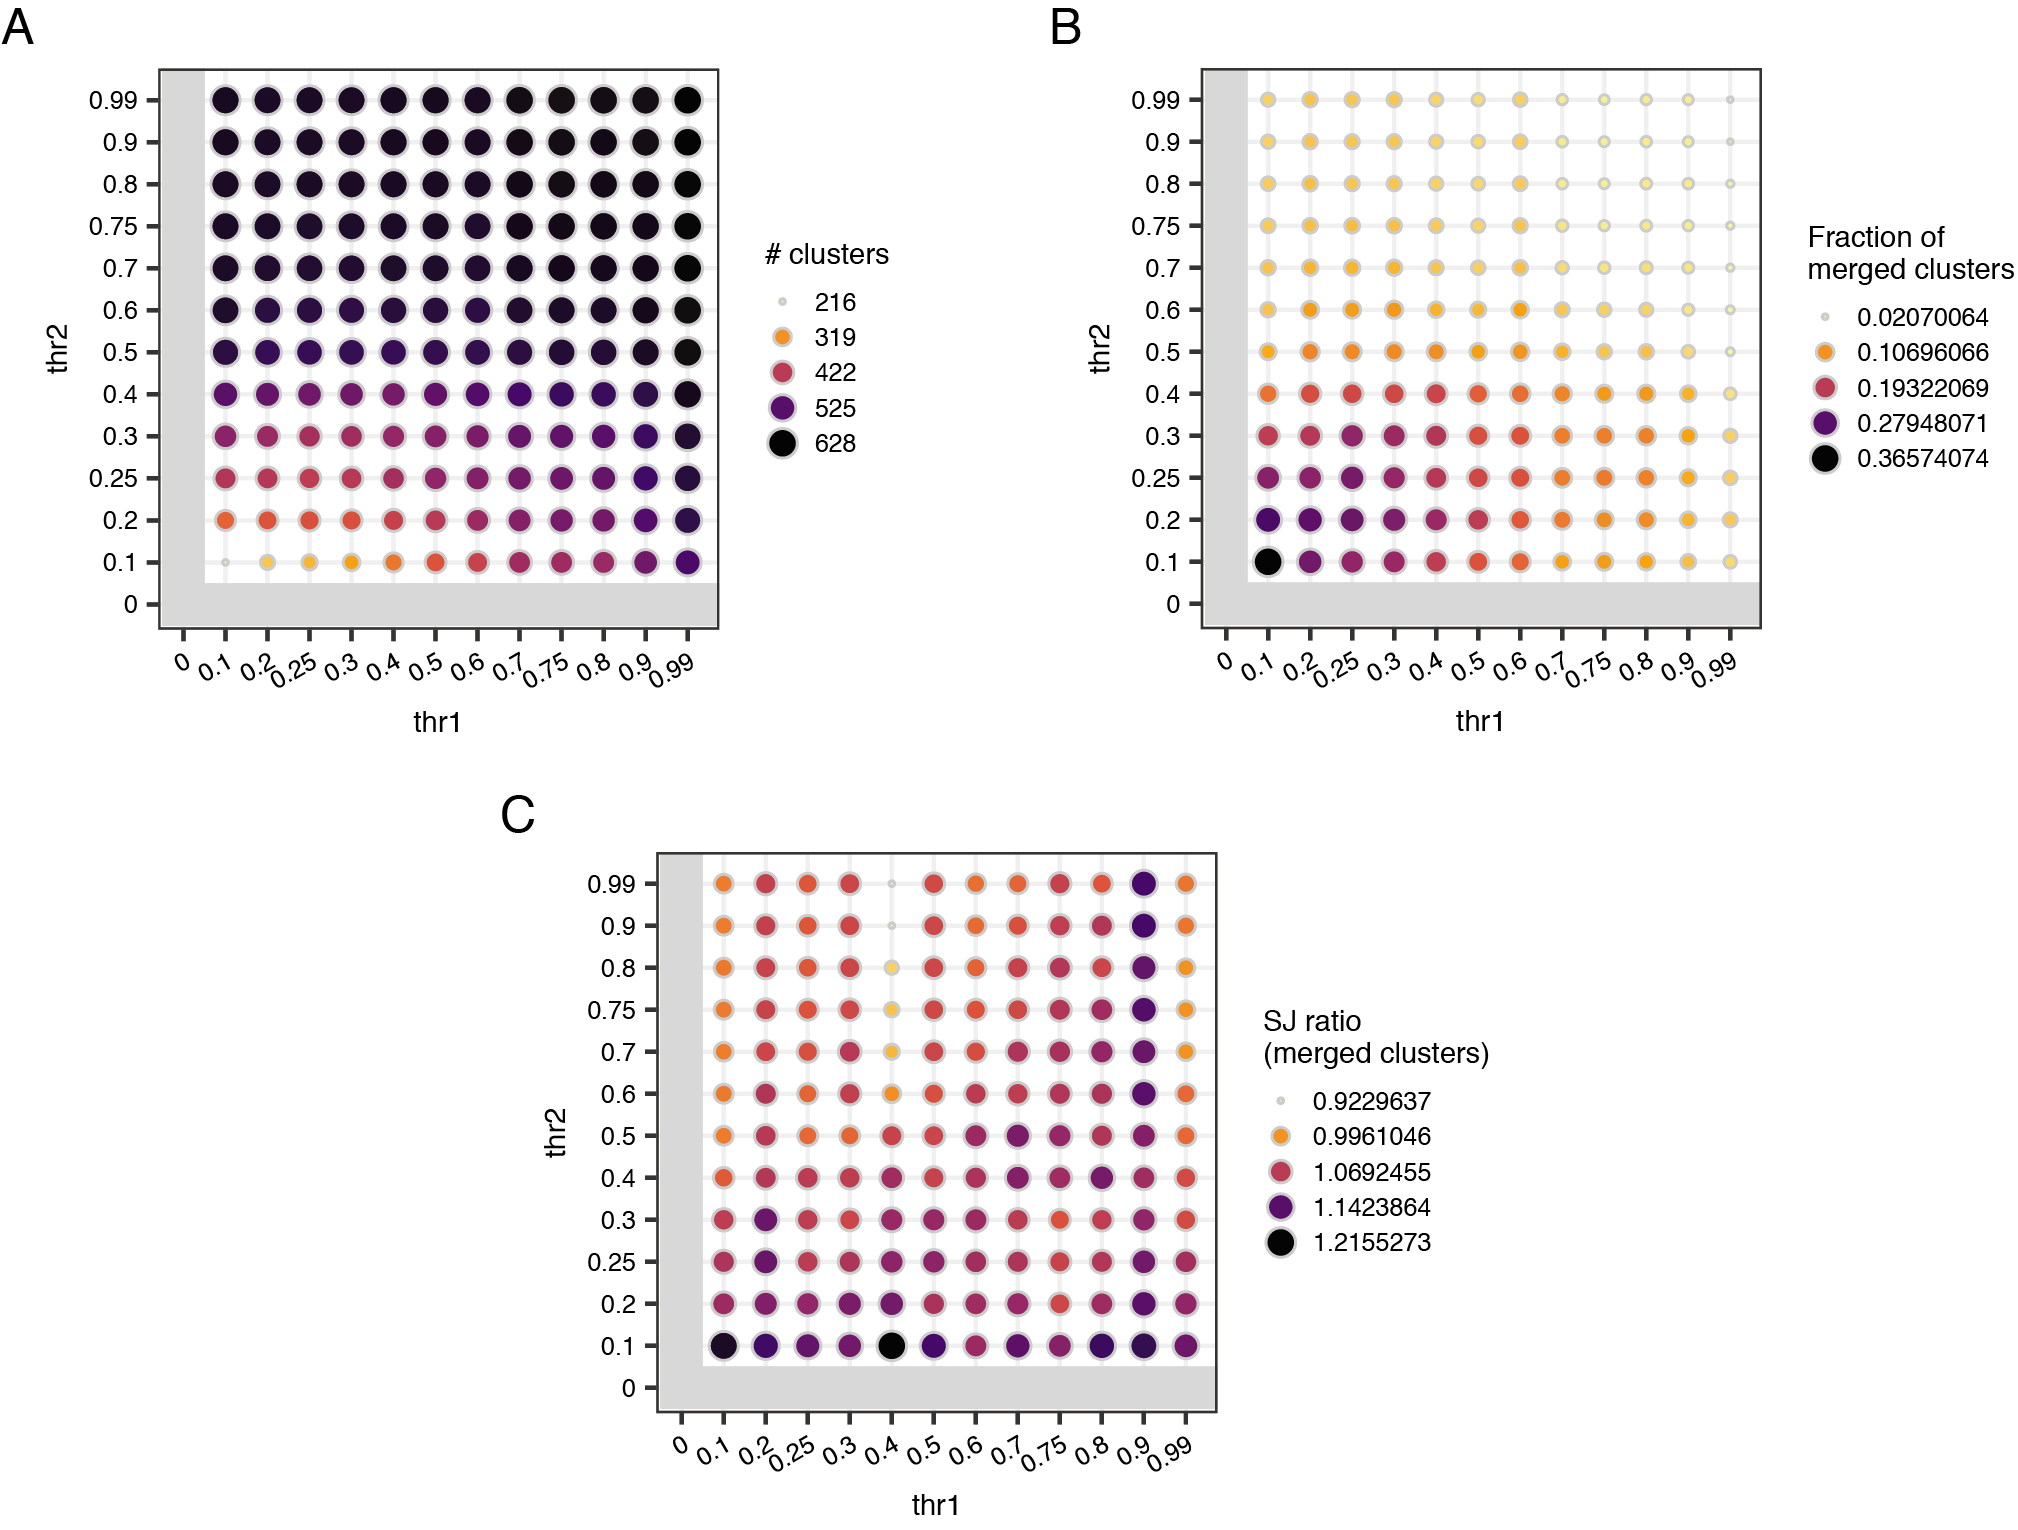
\includegraphics[width=1.0\textwidth]{Appendix2/Figs/chap4_grids.png} % change word in curlies to change figure
\caption[\textit{CellTypist} parameters grids with other statistics]{\textbf{\textit{CellTypist} parameters grids with other statistics (Related to Figure~\ref{fig:chap3_HA})}\newline Parameter grids for \textit{CellTypist} showing variation in \textbf{(A)} total number of clusters; \textbf{(B)} fraction of merged clusters; \textbf{(C)} SJ ratio calculated only for merged clusters.}
\label{fig:appB_grids}
\end{figure}


\begin{figure}[ht!] 
\centering    
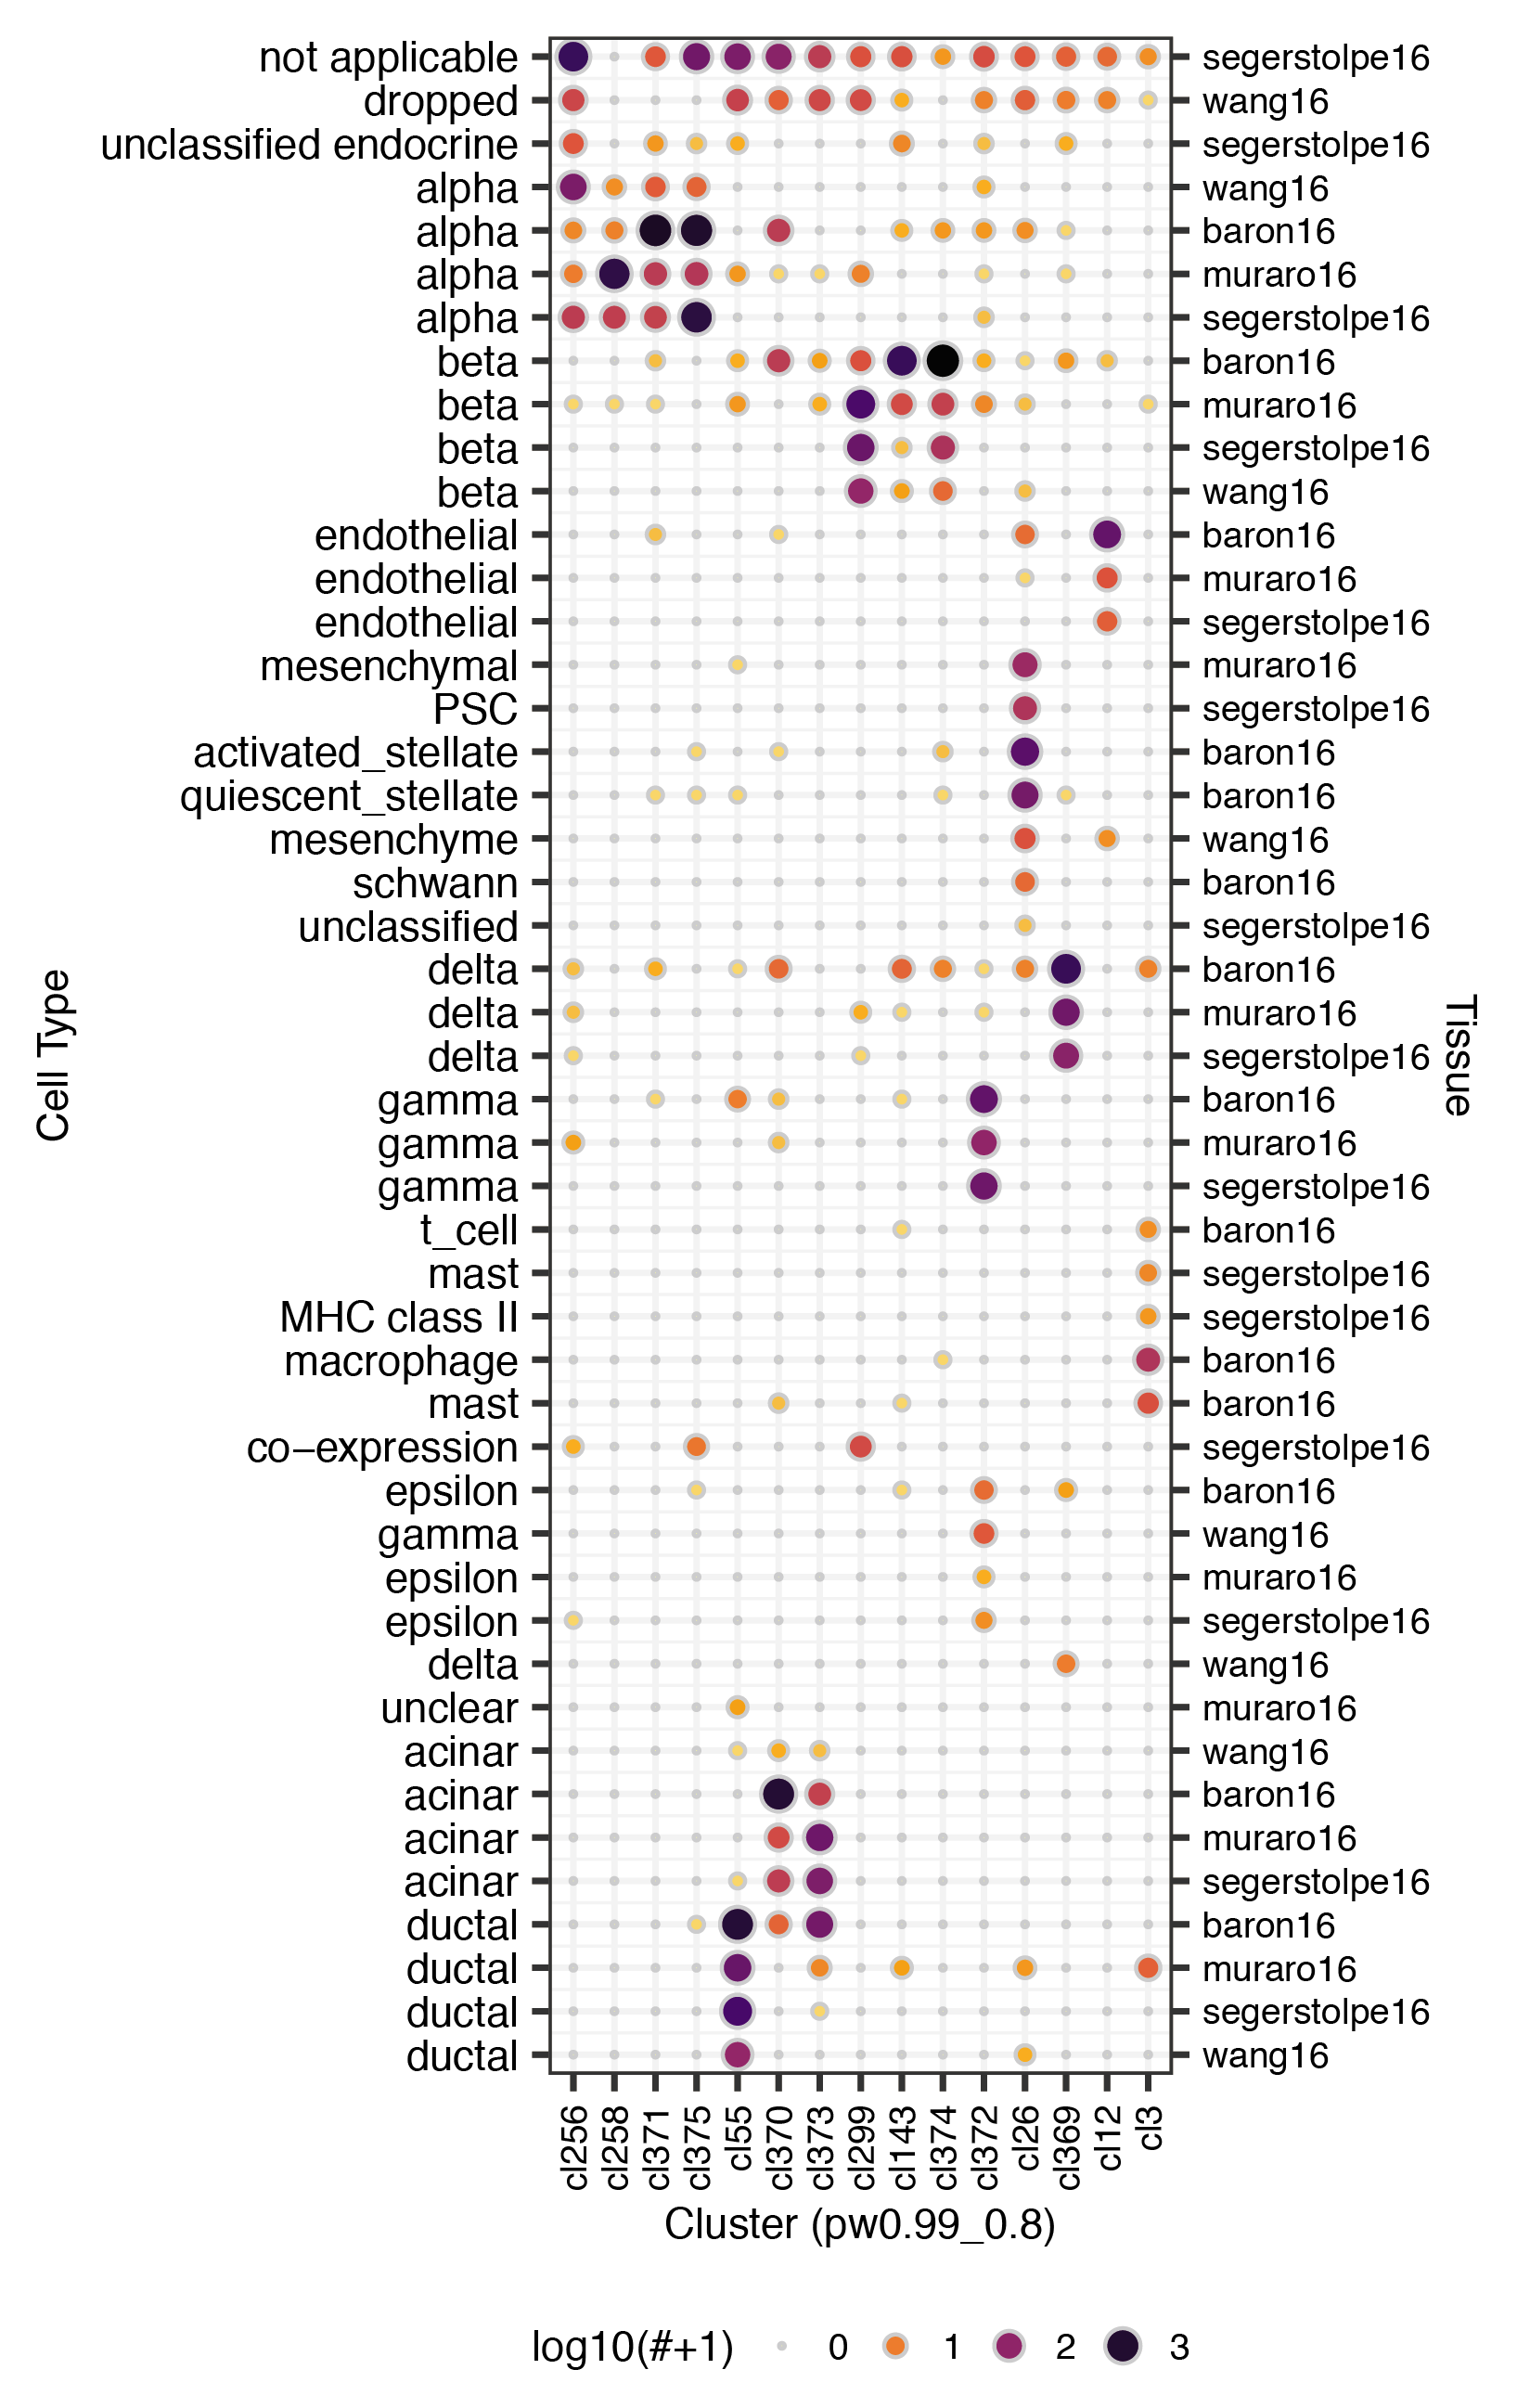
\includegraphics[scale=0.85]{Appendix2/Figs/appB_ctclpancreas.png} % change word in curlies to change figure
\caption[Grouping of annotated cell types and datasets in human pancreas data]{\textbf{Grouping of annotated cell types and datasets in human pancreas data (Related to Figure~\ref{fig:chap3_HA})}\newline Number of cells of each cluster coming from a specific dataset (right y-axis), with a particular cell type annotation (left y-axis). Pancreas was used for this example due to the consistent cell type annotations used across datasets. \textit{CellTypist} parameters: thr1 = 0.99; thr2 = 0.8.}
\label{fig:appB_panc}
\end{figure}

\begin{figure}[ht!] 
\centering    
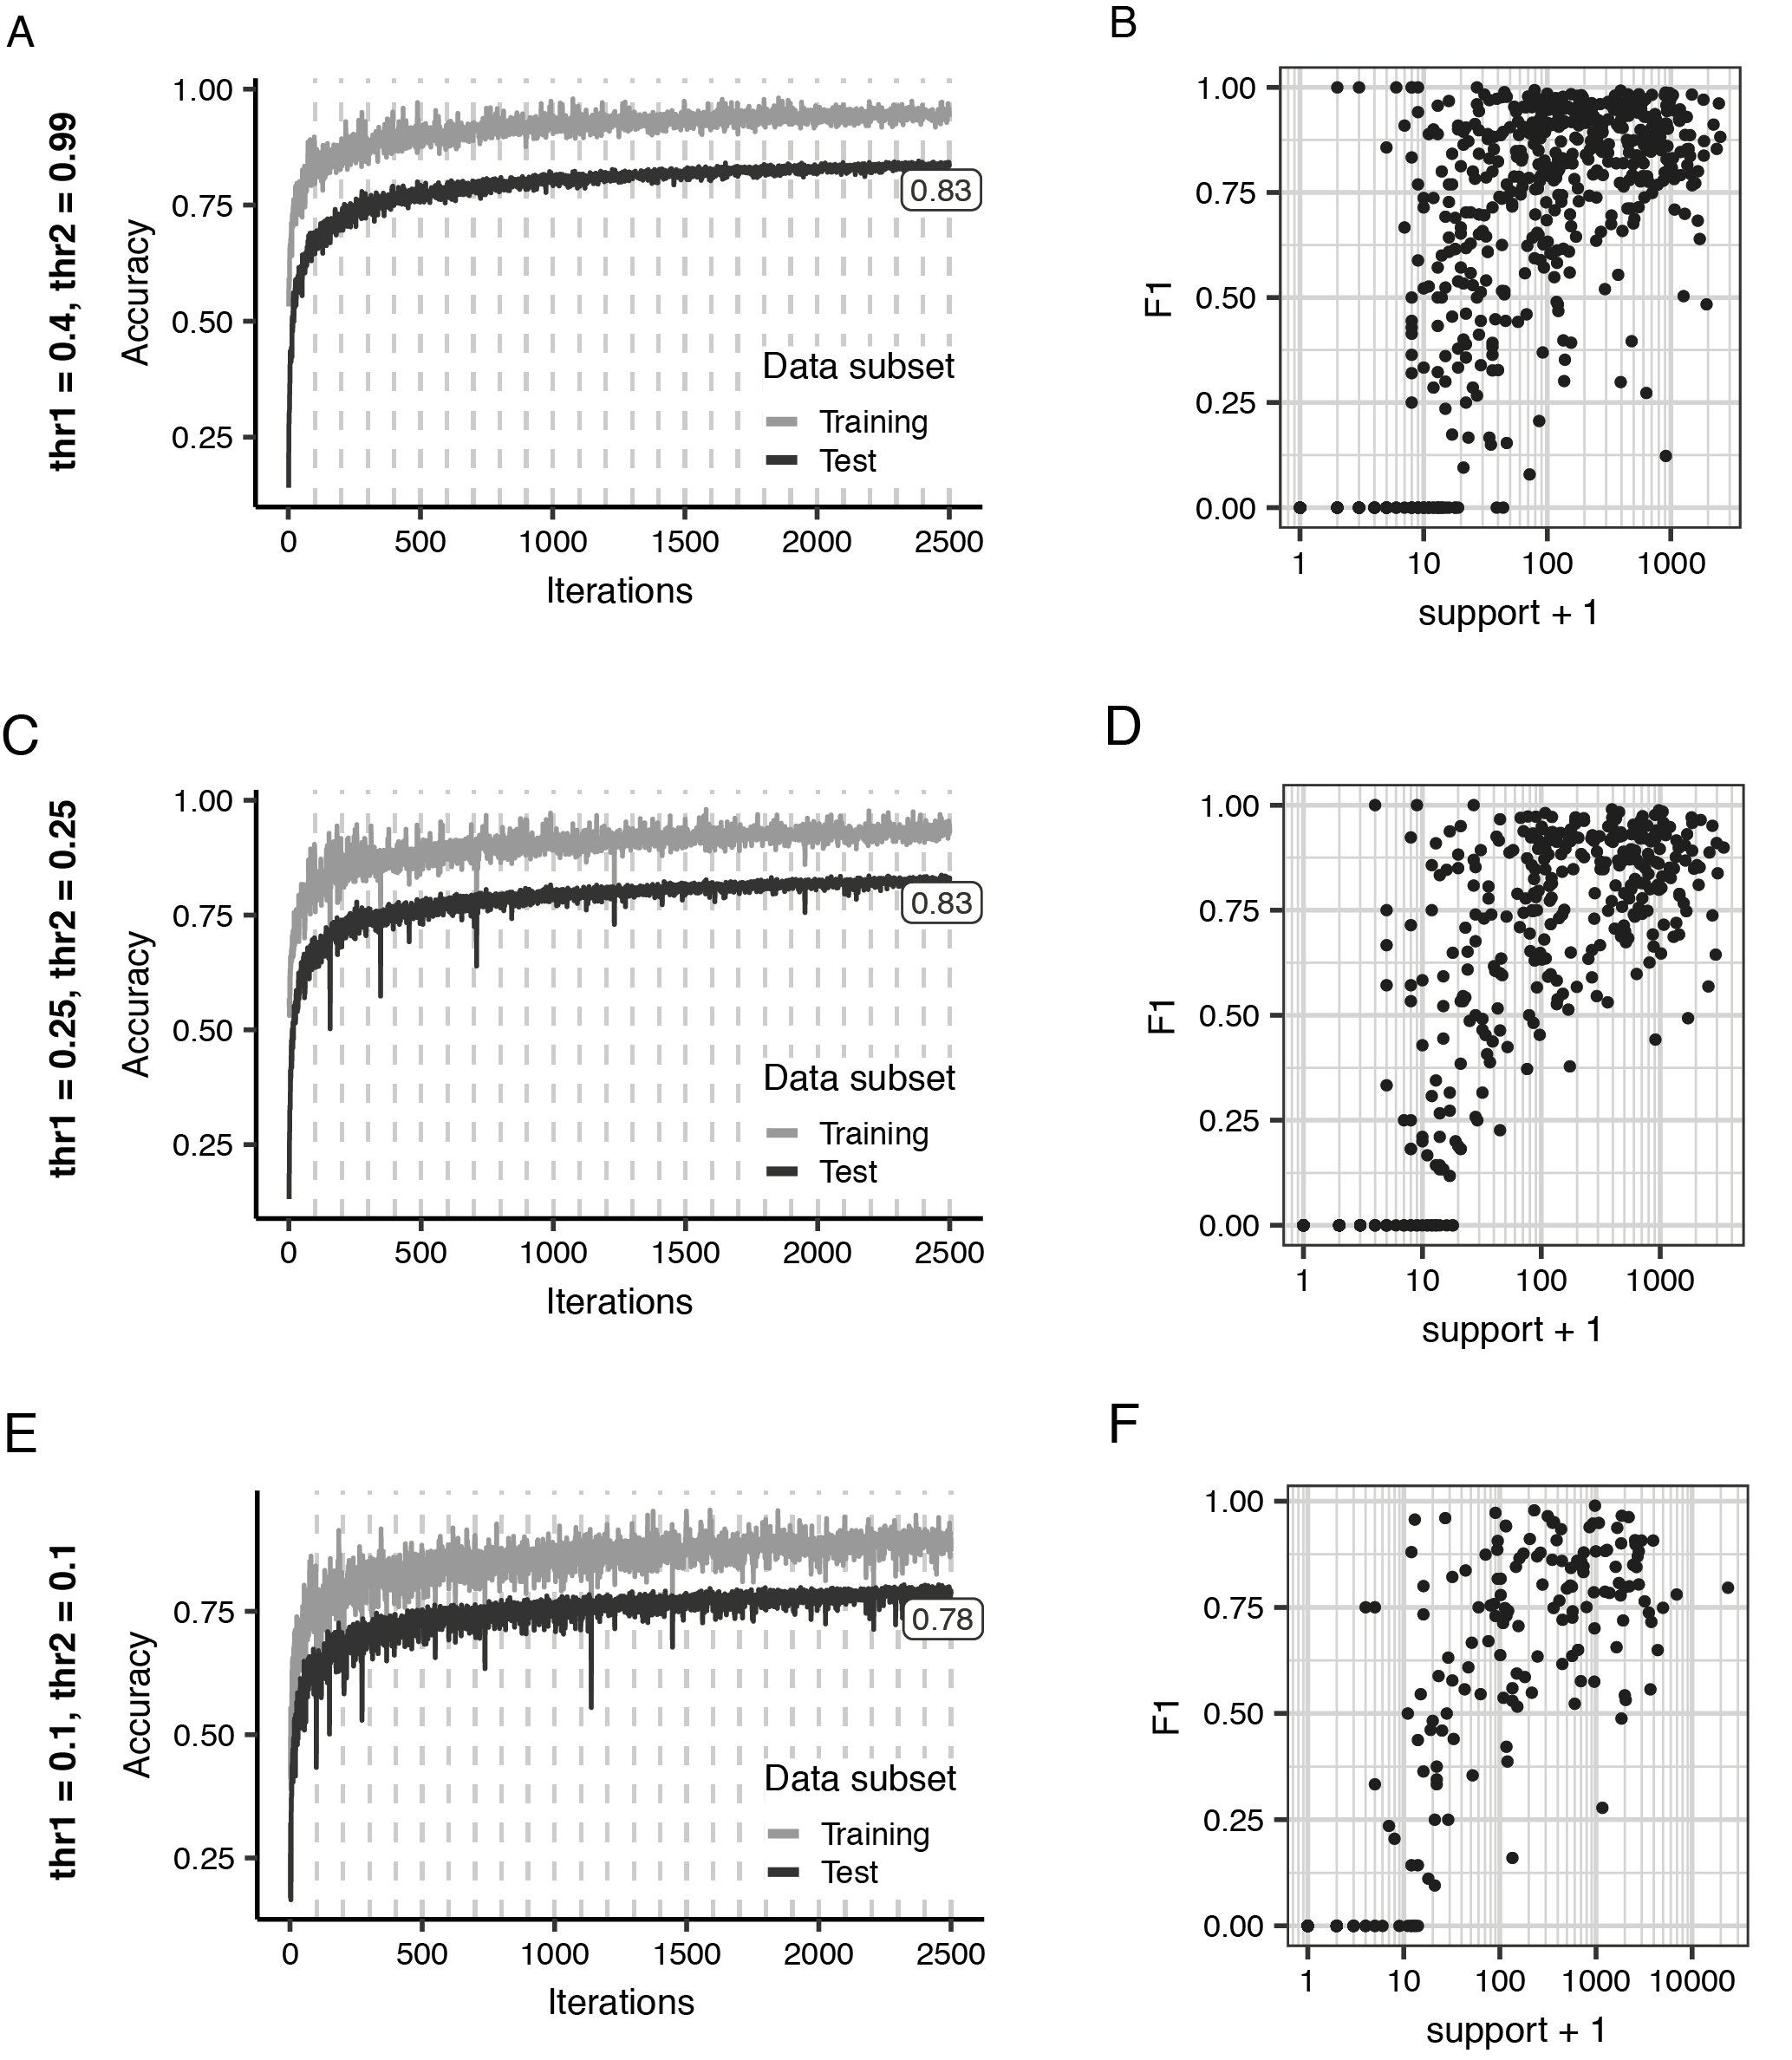
\includegraphics[width=1.0\textwidth]{Appendix2/Figs/appB_modelstuff.png} % change word in curlies to change figure
\caption[Training statistics for other \textit{CellTypist} models]{\textbf{Training statistics for other \textit{CellTypist} models (Related to Figure~\ref{fig:chap3_HA})}\newline For each model trained (thr1 = 0.4 and thr2 = 0.99 - top; thr1 = 0.25 and thr2 = 0.25 - middle; thr1 = 0.1 and thr2 = 0.1 - bottom): \textbf{(A, C, E)} accuracy during model fitting for training and held-out test data; \textbf{(B, D, F)} F1-score for each cluster label (black dots) as a function of class size (in log10 scale).}
\label{fig:appB_moremodels}
\end{figure}


\section{Supplementary Tables}
\label{sectionB1.2}

\begin{table}[pht!]
\small
\caption[F1 scores and class sizes for \textit{CellTypist} trained on the \textit{Tabula Muris} with cell type labels]{F1 scores and class sizes for \textit{CellTypist} trained on the \textit{Tabula Muris} with cell type labels}
\centering
\label{table:tab_tmmodelcells}

\begin{tabular}{lrrr}
  \toprule
Cell Type & F1 Score & Support (Test set) & Total Cells \\ 
  \midrule
Bergmann glial cell & 1.00 &   3 &  30 \\ 
  brain pericyte & 1.00 &  13 & 132 \\ 
  \specialcell[t]{Brush cell of epithelium\\proper of large intestine} & 1.00 &   4 &  45 \\ 
  enteroendocrine cell & 1.00 &   2 &  25 \\ 
  mesothelial cell & 1.00 &   3 &  26 \\ 
  neuronal stem cell & 1.00 &   4 &  36 \\ 
  pancreatic ductal cell & 1.00 &  13 & 131 \\ 
  type II pneumocyte & 1.00 &  18 & 183 \\ 
  microglial cell & 1.00 & 433 & 4329 \\ 
  keratinocyte stem cell & 1.00 & 137 & 1371 \\ 
  oligodendrocyte & 1.00 & 119 & 1186 \\ 
  basal cell & 0.99 & 167 & 1668 \\ 
  \specialcell[t]{luminal epithelial cell\\of mammary gland} & 0.99 &  55 & 552 \\ 
  type B pancreatic cell & 0.99 &  41 & 411 \\ 
  chondroblast & 0.99 &  38 & 380 \\ 
  B cell & 0.98 & 1237 & 12382 \\ 
  kidney tubule cell & 0.98 & 218 & 2182 \\ 
  mesenchymal cell & 0.98 & 184 & 1842 \\ 
  stromal cell & 0.98 & 1261 & 12610 \\ 
  skeletal muscle satellite stem cell & 0.98 &  44 & 442 \\ 
  neuron & 0.98 &  20 & 196 \\ 
  oligodendrocyte precursor cell & 0.97 &  20 & 202 \\ 
  mesenchymal stem cell of adipose & 0.97 & 192 & 1924 \\ 
  basal cell of epidermis & 0.97 & 652 & 6520 \\ 
  hematopoietic stem cell & 0.97 & 267 & 2672 \\ 
  hepatocyte & 0.97 & 141 & 1405 \\ 
  skeletal muscle satellite cell & 0.97 &  90 & 895 \\ 
  pancreatic A cell & 0.97 &  29 & 287 \\ 
  epithelial cell & 0.97 & 102 & 1017 \\ 
  astrocyte of the cerebral cortex & 0.96 &  40 & 403 \\ 
  Fraction A pre-pro B cell & 0.96 &  24 & 240 \\ 
  endocardial cell & 0.96 &  24 & 240 \\ 
  T cell & 0.96 & 835 & 8346 \\ 
  keratinocyte & 0.95 & 278 & 2777 \\ 
  epithelial cell of large intestine & 0.95 & 179 & 1793 \\ 
  endothelial cell & 0.95 & 692 & 6914 \\ 
  large intestine goblet cell & 0.95 &  81 & 814 \\ 
   \bottomrule
\end{tabular}
\end{table}


\begin{table}[pht!]
\small
\caption[F1 scores and class sizes for \textit{CellTypist} trained on the \textit{Tabula Muris} with cell type labels (continued)]{F1 scores and class sizes for \textit{CellTypist} trained on the \textit{Tabula Muris} with cell type labels (continued)}
\centering
\label{table:tab_tmmodelcells2}

\begin{tabular}{lrrr}
  \toprule
Cell Type & F1 Score & Support (Test set) & Total Cells \\ 
  \midrule
fibroblast & 0.95 & 248 & 2487 \\ 
  pancreatic D cell & 0.95 &   9 &  91 \\ 
  pancreatic acinar cell & 0.94 &  18 & 177 \\ 
  \specialcell[t]{enterocyte of epithelium\\of large intestine} & 0.94 &  78 & 782 \\ 
  luminal cell of lactiferous duct & 0.93 &  43 & 430 \\ 
  neutrophil & 0.93 &  82 & 820 \\ 
  mesenchymal stem cell & 0.93 & 163 & 1630 \\ 
  endothelial cell of hepatic sinusoid & 0.92 &  20 & 196 \\ 
  epidermal cell & 0.92 &  45 & 445 \\ 
  granulocyte & 0.91 & 156 & 1559 \\ 
  monocyte & 0.91 & 106 & 1056 \\ 
  neuroendocrine cell & 0.90 &  54 & 543 \\ 
  Kupffer cell & 0.89 &   5 &  51 \\ 
  fenestrated cell & 0.88 &  41 & 414 \\ 
  cardiac muscle cell & 0.87 &  22 & 223 \\ 
  smooth muscle cell & 0.87 &  37 & 367 \\ 
  natural killer cell & 0.85 & 117 & 1168 \\ 
  macrophage & 0.85 & 194 & 1924 \\ 
  leukocyte & 0.84 & 187 & 1878 \\ 
  bladder cell & 0.84 & 146 & 1455 \\ 
  erythrocyte & 0.81 &  21 & 208 \\ 
  ciliated cell & 0.80 &   5 &  55 \\ 
  ciliated epithelial cell & 0.80 &   2 &  20 \\ 
  pancreatic stellate cell & 0.80 &   3 &  29 \\ 
  myeloid cell & 0.79 &  53 & 527 \\ 
  pancreatic PP cell & 0.78 &  11 & 107 \\ 
  kidney collecting duct cell & 0.76 &  12 & 116 \\ 
  stem cell of epidermis & 0.75 &   4 &  45 \\ 
  dendritic cell & 0.71 &  43 & 438 \\ 
  unknown & 0.67 &  63 & 625 \\ 
  Clara cell & 0.67 &   2 &  18 \\ 
  hematopoietic cell & 0.67 &   2 &  17 \\ 
  mast cell & 0.44 &   2 &  22 \\ 
  basal cell of urothelium & 0.40 &  36 & 365 \\ 
  basal cell of epithelium of trachea & 0.12 &   4 &  36 \\ 
  epicardial adipocyte & 0.00 &   9 &  93 \\ 
  lung neuroendocrine cell & 0.00 &   0 &   2 \\ 
  type I pneumocyte & 0.00 &   0 &   2 \\ 
   \bottomrule
\end{tabular}
\end{table}

\begin{table}[ht!]
\scriptsize
\caption[F1 scores and class sizes for \textit{CellTypist} trained on the \textit{Tabula Muris} with integrated cluster labels]{F1 scores and class sizes for \textit{CellTypist} trained on the \textit{Tabula Muris} with integrated cluster labels}
\centering
\label{table:tab_tmmodelclust}
\begin{tabular}{lrrrll}
  \toprule
Cluster & F1 Score & Test Support & Total Cells & Major Cell Type & Major Tissue \\
  \midrule
cl103 & 1.00 &  21 & 207 & endothelial cell (93.7\%) & Lung (100\%) \\ 
  cl124 & 1.00 &   8 &  82 & neuron (100\%) & Brain\_Neurons (100\%) \\ 
  cl135 & 1.00 &   3 &  26 & neuron (100\%) & Brain\_Neurons (100\%) \\ 
  cl138 & 1.00 &   6 &  57 & neuron (98.2\%) & Brain\_Neurons (100\%) \\ 
  cl147 & 1.00 &  15 & 147 & kidney collecting duct cell (57.1\%) & Kidney (100\%) \\ 
  cl154 & 1.00 &   2 &  17 & neuron (100\%) & Brain\_Neurons (100\%) \\ 
  cl166 & 1.00 &   5 &  50 & type B pancreatic cell (100\%) & Pancreas (100\%) \\ 
  cl175 & 1.00 &  10 &  96 & Fraction A pre-pro B cell (65.6\%) & Marrow (100\%) \\ 
  cl185 & 1.00 &   5 &  47 & \specialcell[t]{Brush cell of epithelium proper\\of large intestine (89.4\%) } & Colon (100\%) \\ 
  cl186 & 1.00 &   1 &   8 & neuron (100\%) & Brain\_Neurons (100\%) \\ 
  cl189 & 1.00 &  46 & 462 & hepatocyte (97.4\%) & Liver (100\%) \\ 
  cl193 & 1.00 &   4 &  39 & unknown (61.5\%) & Aorta (100\%) \\ 
  cl194 & 1.00 &   1 &  14 & enteroendocrine cell (100\%) & Colon (100\%) \\ 
  cl20 & 1.00 &  12 & 123 & pancreatic ductal cell (99.2\%) & Pancreas (100\%) \\ 
  cl27 & 1.00 &   1 &   9 & enteroendocrine cell (100\%) & Colon (100\%) \\ 
  cl65 & 1.00 &   2 &  21 & pancreatic stellate cell (90.5\%) & Pancreas (100\%) \\ 
  cl73 & 1.00 &   2 &  21 & leukocyte (100\%) & Pancreas (100\%) \\ 
  cl89 & 1.00 &   1 &  13 & \specialcell[t]{astrocyte of the\\cerebral cortex (69.2\%)} & Brain\_Neurons (69.2\%) \\ 
  cl161 & 0.99 &  96 & 959 & keratinocyte (93.8\%) & Tongue (100\%) \\ 
  cl150 & 0.99 &  83 & 833 & keratinocyte stem cell (97.7\%) & Skin (100\%) \\ 
  cl70 & 0.99 & 163 & 1631 & basal cell (99.8\%) & Mammary (100\%) \\ 
  cl157 & 0.99 &  68 & 682 & \specialcell[t]{luminal epithelial cell\\of mammary gland (57.8\%)} & Mammary (100\%) \\ 
  cl190 & 0.99 &  58 & 583 & hepatocyte (100\%) & Liver (100\%) \\ 
  cl143 & 0.99 &  54 & 544 & kidney tubule cell (98\%) & Kidney (100\%) \\ 
  cl171 & 0.99 &  54 & 539 & keratinocyte stem cell (99.6\%) & Skin (100\%) \\ 
  cl26 & 0.99 &  36 & 357 & luminal cell of lactiferous duct (51\%) & Mammary (100\%) \\ 
  cl81 & 0.99 &  72 & 715 & endothelial cell (93.3\%) & Lung (100\%) \\ 
  cl38 & 0.98 & 223 & 2227 & fibroblast (99.3\%) & Heart (100\%) \\ 
  cl100 & 0.98 & 105 & 1052 & mesenchymal cell (97.1\%) & Bladder (100\%) \\ 
  cl108 & 0.98 &  49 & 494 & epithelial cell (54.5\%) & Trachea (55.9\%) \\ 
  cl31 & 0.98 & 496 & 4961 & stromal cell (97.4\%) & Trachea (100\%) \\ 
  cl49 & 0.98 &  82 & 823 & mesenchymal cell (98.4\%) & Bladder (100\%) \\ 
  cl122 & 0.97 &  39 & 386 & stromal cell (99.7\%) & Lung (100\%) \\ 
  cl37 & 0.97 & 367 & 3665 & stromal cell (98.4\%) & Trachea (100\%) \\ 
  cl17 & 0.97 &  74 & 742 & \specialcell[t]{epithelial cell of\\large intestine (99.9\%)} & Colon (100\%) \\ 
  cl95 & 0.97 &  90 & 899 & T cell (99.8\%) & Thymus (100\%) \\ 
  cl6 & 0.97 & 227 & 2267 & hematopoietic stem cell (73.7\%) & Marrow (100\%) \\ 
  cl165 & 0.97 & 101 & 1008 & kidney tubule cell (98.5\%) & Kidney (100\%) \\ 
  cl47 & 0.97 & 116 & 1157 & bladder cell (78\%) & Bladder (100\%) \\ 
  cl1 & 0.97 & 454 & 4543 & basal cell of epidermis (95\%) & Tongue (100\%) \\ 
  cl54 & 0.97 & 180 & 1798 & granulocyte (61.5\%) & Marrow (100\%) \\ 
  cl136 & 0.97 &  63 & 631 & T cell (100\%) & Thymus (100\%) \\ 
  cl24 & 0.97 &  63 & 631 & epithelial cell (92.4\%) & Trachea (100\%) \\ 
  cl106 & 0.96 &  41 & 407 & chondroblast (93.1\%) & Muscle (99.3\%) \\ 
  cl180 & 0.96 &  39 & 392 & kidney tubule cell (98.7\%) & Kidney (100\%) \\ 
  cl141 & 0.96 & 128 & 1279 & \specialcell[t]{skeletal muscle\\satellite cell (67.9\%)} & Muscle (70\%) \\ 
  cl71 & 0.96 &  24 & 239 & smooth muscle cell (98.7\%) & Heart (100\%) \\ 
  cl32 & 0.96 &  24 & 238 & mesenchymal stem cell (97.5\%) & Diaphragm (100\%) \\ 
  cl85 & 0.96 &  82 & 822 & natural killer cell (99.8\%) & Lung (100\%) \\ 
  cl44 & 0.96 & 143 & 1434 & mesenchymal stem cell (93.4\%) & Muscle (100\%) \\ 
  cl176 & 0.96 &  24 & 242 & \specialcell[t]{enterocyte of epithelium of\\large intestine (97.9\%)} & Colon (100\%) \\ 
  cl181 & 0.96 &  23 & 229 & \specialcell[t]{astrocyte ofthe\\cerebral cortex (92.6\%)} & Brain\_Neurons (100\%) \\ 
  cl76 & 0.95 &  23 & 232 & endocardial cell (98.7\%) & Heart (100\%) \\ 
  cl151 & 0.95 &  32 & 324 & hepatocyte (99.7\%) & Liver (100\%) \\ 
   \bottomrule
\end{tabular}
\end{table}

\begin{table}[ht!]
\scriptsize
\caption[F1 scores and class sizes for \textit{CellTypist} trained on the \textit{Tabula Muris} with integrated cluster labels (continued 1)]{F1 scores and class sizes for \textit{CellTypist} trained on the \textit{Tabula Muris} with integrated cluster labels (continued 1)}
\centering
\label{table:tab_tmmodelclust1}
\begin{tabular}{lrrrll}
  \toprule
Cluster & F1 Score & Test Support & Total Cells & Major Cell Type & Major Tissue \\
  \midrule
  cl126 & 0.95 &  22 & 223 & keratinocyte (95.5\%) & Tongue (100\%) \\ 
  cl39 & 0.95 & 159 & 1593 & endothelial cell (72.8\%) & Trachea (65.3\%) \\ 
  cl99 & 0.95 &  87 & 868 & stromal cell (99.1\%) & Lung (100\%) \\ 
  cl140 & 0.95 &  68 & 684 & hematopoietic stem cell (64\%) & Marrow (100\%) \\ 
  cl83 & 0.95 &  38 & 379 & macrophage (53.6\%) & Marrow (98.2\%) \\ 
  cl187 & 0.95 &  19 & 188 & type II pneumocyte (97.3\%) & Lung (100\%) \\ 
  cl159 & 0.94 &  17 & 174 & \specialcell[t]{oligodendrocyte precursor\\cell (99.4\%)} & Brain\_Neurons (100\%) \\ 
  cl62 & 0.94 & 196 & 1955 & endothelial cell (98.7\%) & Heart (68\%) \\ 
  cl86 & 0.94 & 101 & 1012 & basal cell of epidermis (95.6\%) & Tongue (99.4\%) \\ 
  cl125 & 0.94 &  17 & 168 & type B pancreatic cell (98.2\%) & Pancreas (100\%) \\ 
  cl144 & 0.94 &  77 & 771 & basal cell of epidermis (95.2\%) & Tongue (100\%) \\ 
  cl64 & 0.94 & 150 & 1504 & T cell (99.1\%) & Mammary (100\%) \\ 
  cl48 & 0.94 &  68 & 678 & stromal cell (99\%) & Mammary (100\%) \\ 
  cl131 & 0.94 &  86 & 862 & oligodendrocyte (96.6\%) & Brain\_Neurons (100\%) \\ 
  cl60 & 0.94 & 239 & 2391 & T cell (99.3\%) & Spleen (100\%) \\ 
  cl74 & 0.94 & 753 & 7534 & B cell (98.6\%) & Spleen (70.5\%) \\ 
  cl14 & 0.94 & 123 & 1232 & B cell (60\%) & Mammary (100\%) \\ 
  cl110 & 0.94 &  63 & 630 & bladder cell (81.4\%) & Bladder (99.4\%) \\ 
  cl18 & 0.94 &  97 & 965 & leukocyte (97.3\%) & Trachea (100\%) \\ 
  cl96 & 0.94 &  73 & 729 & \specialcell[t]{mesenchymal stem cell\\of adipose (55.4\%)} & Fat (55.7\%) \\ 
  cl55 & 0.94 & 132 & 1318 & endothelial cell (98\%) & Muscle (100\%) \\ 
  cl113 & 0.94 & 143 & 1434 & keratinocyte (97.6\%) & Tongue (99.7\%) \\ 
  cl132 & 0.94 &  23 & 226 & \specialcell[t]{epithelial cell of\\large intestine (83.2\%)} & Colon (100\%) \\ 
  cl43 & 0.93 & 120 & 1197 & monocyte (69.2\%) & Marrow (100\%) \\ 
  cl112 & 0.93 &   8 &  84 & large intestine goblet cell (100\%) & Colon (100\%) \\ 
  cl97 & 0.93 &   8 &  80 & \specialcell[t]{mesenchymal stem cell\\of adipose (100\%)} & Fat (100\%) \\ 
  cl173 & 0.93 &  22 & 220 & epidermal cell (93.2\%) & Skin (100\%) \\ 
  cl67 & 0.93 &  29 & 294 & granulocyte (94.6\%) & Fat (100\%) \\ 
  cl129 & 0.93 &  36 & 360 & stromal cell (99.2\%) & Lung (100\%) \\ 
  cl0 & 0.93 & 118 & 1182 & T cell (87.9\%) & Thymus (100\%) \\ 
  cl127 & 0.93 &  35 & 348 & large intestine goblet cell (87.9\%) & Colon (100\%) \\ 
  cl35 & 0.92 &  48 & 481 & leukocyte (88.4\%) & Heart (100\%) \\ 
  cl82 & 0.92 &  18 & 179 & brain pericyte (58.1\%) & Brain\_Neurons (58.1\%) \\ 
  cl21 & 0.92 &  31 & 307 & endothelial cell (94.8\%) & Mammary (100\%) \\ 
  cl57 & 0.92 &  54 & 537 & B cell (98.7\%) & Muscle (100\%) \\ 
  cl11 & 0.91 &  11 & 115 & ciliated cell (47\%) & Lung (100\%) \\ 
  cl58 & 0.91 &  21 & 211 & \specialcell[t]{endothelial cell of\\hepatic sinusoid (85.8\%)} & Liver (100\%) \\ 
  cl121 & 0.90 &  41 & 413 & \specialcell[t]{epithelial cell of\\large intestine (99.8\%)} & Colon (100\%) \\ 
  cl42 & 0.90 &  20 & 204 & neuroendocrine cell (95.1\%) & Trachea (100\%) \\ 
  cl88 & 0.90 &  31 & 308 & myeloid cell (99\%) & Fat (100\%) \\ 
  cl52 & 0.90 &  54 & 538 & endothelial cell (99.3\%) & Fat (100\%) \\ 
  cl184 & 0.89 &  12 & 117 & pancreatic acinar cell (97.4\%) & Pancreas (100\%) \\ 
  cl34 & 0.89 &  33 & 327 & macrophage (96.9\%) & Muscle (100\%) \\ 
  cl130 & 0.89 &  18 & 176 & large intestine goblet cell (96\%) & Colon (100\%) \\ 
  cl72 & 0.89 &  94 & 938 & \specialcell[t]{mesenchymal stem cell\\of adipose (99.9\%)} & Fat (100\%) \\ 
  cl94 & 0.89 &  62 & 617 & stromal cell (97.4\%) & Lung (100\%) \\ 
  cl142 & 0.88 &  16 & 156 & type B pancreatic cell (100\%) & Pancreas (100\%) \\ 
  cl77 & 0.88 &  31 & 309 & leukocyte (48.9\%) & Lung (58.3\%) \\ 
  cl13 & 0.88 &  33 & 326 & unknown (61\%) & Muscle (100\%) \\ 
  cl145 & 0.88 &  38 & 384 & basal cell of epidermis (80.7\%) & Skin (100\%) \\ 
  cl45 & 0.88 &  55 & 545 & stromal cell (94.3\%) & Lung (100\%) \\ 
  cl102 & 0.87 &  17 & 170 & stromal cell (87.6\%) & Lung (97.1\%) \\ 
   \bottomrule
\end{tabular}
\end{table}

\begin{table}[ht!]
\scriptsize
\caption[F1 scores and class sizes for \textit{CellTypist} trained on the \textit{Tabula Muris} with integrated cluster labels (continued 2)]{F1 scores and class sizes for \textit{CellTypist} trained on the \textit{Tabula Muris} with integrated cluster labels (continued 2)}
\centering
\label{table:tab_tmmodelclust2}
\begin{tabular}{lrrrll}
  \toprule
Cluster & F1 Score & Test Support & Total Cells & Major Cell Type & Major Tissue \\
  \midrule
  cl153 & 0.87 &  14 & 137 & pancreatic A cell (71.5\%) & Pancreas (100\%) \\ 
  cl84 & 0.86 &  22 & 216 & monocyte (81.9\%) & Lung (100\%) \\ 
  cl15 & 0.86 &  24 & 239 & macrophage (74.9\%) & Kidney (100\%) \\ 
  cl51 & 0.86 & 123 & 1229 & microglial cell (99.6\%) & Brain\_Microglia (100\%) \\ 
  cl172 & 0.86 &  18 & 177 & large intestine goblet cell (52\%) & Colon (100\%) \\ 
  cl87 & 0.86 &  29 & 294 & dendritic cell (88.4\%) & Lung (100\%) \\ 
  cl90 & 0.86 &   8 &  76 & endothelial cell (100\%) & Aorta (100\%) \\ 
  cl10 & 0.85 & 271 & 2706 & B cell (98.1\%) & Spleen (100\%) \\ 
  cl7 & 0.85 &  53 & 535 & macrophage (63.6\%) & Spleen (100\%) \\ 
  cl177 & 0.85 &  21 & 208 & \specialcell[t]{enterocyte of epithelium of\\large intestine (90.4\%)} & Colon (100\%) \\ 
  cl53 & 0.83 &  27 & 273 & endothelial cell (96.3\%) & Lung (100\%) \\ 
  cl183 & 0.83 &  13 & 128 & large intestine goblet cell (98.4\%) & Colon (100\%) \\ 
  cl29 & 0.83 & 170 & 1700 & microglial cell (100\%) & Brain\_Microglia (100\%) \\ 
  cl162 & 0.83 &  24 & 237 & \specialcell[t]{enterocyte of epithelium of\\large intestine (98.7\%)} & Colon (100\%) \\ 
  cl115 & 0.83 &  22 & 219 & \specialcell[t]{mesenchymal stem cell\\of adipose (99.5\%)} & Fat (100\%) \\ 
  cl188 & 0.83 &  20 & 197 & \specialcell[t]{astrocyte of the\\cerebral cortex (87.3\%)} & Brain\_Neurons (100\%) \\ 
  cl119 & 0.83 &  32 & 317 & oligodendrocyte (99.7\%) & Brain\_Neurons (100\%) \\ 
  cl40 & 0.83 &  26 & 260 & neuroendocrine cell (74.2\%) & Trachea (100\%) \\ 
  cl107 & 0.82 &   9 &  94 & epidermal cell (43.6\%) & Skin (96.8\%) \\ 
  cl109 & 0.82 &  26 & 265 & \specialcell[t]{mesenchymal stem cell\\of adipose (100\%)} & Fat (100\%) \\ 
  cl12 & 0.81 & 143 & 1427 & microglial cell (98.5\%) & Brain\_Microglia (100\%) \\ 
  cl152 & 0.81 &  15 & 155 & pancreatic A cell (98.1\%) & Pancreas (100\%) \\ 
  cl56 & 0.80 &  47 & 467 & T cell (72.8\%) & Fat (100\%) \\ 
  cl9 & 0.80 &   5 &  49 & epithelial cell (95.9\%) & Fat (100\%) \\ 
  cl69 & 0.80 &  11 & 113 & neuroendocrine cell (90.3\%) & Trachea (100\%) \\ 
  cl80 & 0.79 &  22 & 222 & neutrophil (98.2\%) & Fat (100\%) \\ 
  cl36 & 0.79 &  16 & 162 & myeloid cell (90.1\%) & Fat (100\%) \\ 
  cl149 & 0.79 &  19 & 186 & epidermal cell (57.5\%) & Skin (100\%) \\ 
  cl68 & 0.79 &  77 & 766 & T cell (74.7\%) & Marrow (60.8\%) \\ 
  cl191 & 0.78 &  13 & 131 & epithelial cell of large intestine (59.5\%) & Colon (100\%) \\ 
  cl63 & 0.77 &  31 & 315 & T cell (91.1\%) & Lung (100\%) \\ 
  cl2 & 0.77 &  16 & 156 & Kupffer cell (32.7\%) & Liver (100\%) \\
  cl158 & 0.77 &  25 & 255 & epithelial cell of large intestine (76.1\%) & Colon (100\%) \\ 
  cl197 & 0.76 &  10 &  97 & unknown (58.8\%) & Brain\_Neurons (100\%) \\ 
  cl114 & 0.75 &  35 & 354 & macrophage (99.4\%) & Lung (100\%) \\ 
  cl28 & 0.75 &   9 &  94 & B cell (69.1\%) & Diaphragm (100\%) \\ 
  cl101 & 0.75 &   5 &  48 & endothelial cell (93.8\%) & Fat (91.7\%) \\ 
  cl111 & 0.75 &   5 &  53 & oligodendrocyte (64.2\%) & Brain\_Neurons (100\%) \\ 
  cl4 & 0.71 &  31 & 313 & cardiac muscle cell (62.9\%) & Heart (100\%) \\ 
  cl5 & 0.70 &  21 & 210 & fibroblast (66.2\%) & Kidney (100\%) \\ 
  cl148 & 0.70 &  11 & 107 & pancreatic D cell (57.9\%) & Pancreas (100\%) \\ 
  cl30 & 0.69 &  36 & 362 & T cell (96.4\%) & Muscle (100\%) \\ 
  cl93 & 0.67 &   1 &   9 & unknown (44.4\%) & Aorta (100\%) \\ 
  cl41 & 0.62 &  19 & 187 & macrophage (73.8\%) & Lung (100\%) \\ 
  cl25 & 0.62 &   6 &  60 & leukocyte (90\%) & Bladder (100\%) \\ 
  cl8 & 0.59 &  11 & 106 & unknown (67.9\%) & Brain\_Neurons (100\%) \\ 
  cl50 & 0.57 &   5 &  46 & fibroblast (58.7\%) & Aorta (100\%) \\ 
  cl33 & 0.55 &   8 &  78 & endothelial cell (92.3\%) & Diaphragm (100\%) \\ 
  cl19 & 0.50 &   1 &  14 & leukocyte (78.6\%) & Pancreas (100\%) \\ 
  cl79 & 0.50 &   3 &  26 & smooth muscle cell (96.2\%) & Fat (100\%) \\ 
  cl16 & 0.48 &   7 &  69 & endothelial cell (85.5\%) & Bladder (100\%) \\ 
  cl66 & 0.45 &  26 & 262 & B cell (98.1\%) & Lung (100\%) \\ 
  cl59 & 0.44 &   4 &  36 & leukocyte (77.8\%) & Kidney (100\%) \\ 
  cl23 & 0.22 &   7 &  67 & epicardial adipocyte (47.8\%) & Aorta (100\%) \\ 
  cl155 & 0.18 &   2 &  18 & pancreatic acinar cell (100\%) & Pancreas (100\%) \\ 
   \bottomrule
\end{tabular}
\end{table}

\begin{table}[ht!]
\scriptsize
\caption[F1 scores and class sizes for \textit{CellTypist} trained on the \textit{Tabula Muris} with integrated cluster labels (continued 3)]{F1 scores and class sizes for \textit{CellTypist} trained on the \textit{Tabula Muris} with integrated cluster labels (continued 3)}
\centering
\label{table:tab_tmmodelclust3}
\begin{tabular}{lrrrll}
  \toprule
Cluster & F1 Score & Test Support & Total Cells & Major Cell Type & Major Tissue \\
  \midrule
  cl104 & 0.00 &   0 &   5 & \specialcell[t]{mesenchymal stem cell\\of adipose (100\%)} & Fat (100\%) \\ 
  cl105 & 0.00 &   0 &   4 & \specialcell[t]{mesenchymal stem cell\\of adipose (100\%)} & Fat (100\%) \\ 
  cl116 & 0.00 &   0 &   5 & endothelial cell (100\%) & Fat (100\%) \\ 
  cl117 & 0.00 &   1 &  12 & smooth muscle cell (100\%) & Brain\_Neurons (100\%) \\ 
  cl118 & 0.00 &   0 &   3 & \specialcell[t]{epithelial cell of\\large intestine (66.7\%)} & Colon (100\%) \\ 
  cl120 & 0.00 &   0 &   5 & endothelial cell (100\%) & Brain\_Neurons (100\%) \\ 
  cl123 & 0.00 &   2 &  16 & pancreatic PP cell (100\%) & Pancreas (100\%) \\ 
  cl128 & 0.00 &   1 &   6 & pancreatic PP cell (100\%) & Pancreas (100\%) \\ 
  cl133 & 0.00 &   1 &   9 & \specialcell[t]{oligodendrocyte precursor\\cell (100\%)} & Brain\_Neurons (100\%) \\ 
  cl134 & 0.00 &   0 &   4 & \specialcell[t]{epithelial cell of\\large intestine (100\%)} & Colon (100\%) \\ 
  cl137 & 0.00 &   1 &  14 & pancreatic A cell (64.3\%) & Pancreas (100\%) \\ 
  cl139 & 0.00 &   3 &  34 & pancreatic A cell (64.7\%) & Pancreas (100\%) \\ 
  cl146 & 0.00 &   1 &   9 & T cell (88.9\%) & Fat (100\%) \\ 
  cl156 & 0.00 &   3 &  26 & pancreatic D cell (100\%) & Pancreas (100\%) \\ 
  cl160 & 0.00 &   1 &   8 & type B pancreatic cell (100\%) & Pancreas (100\%) \\ 
  cl163 & 0.00 &   0 &   3 & type B pancreatic cell (100\%) & Pancreas (100\%) \\ 
  cl164 & 0.00 &   0 &   4 & neuron (100\%) & Brain\_Neurons (100\%) \\ 
  cl167 & 0.00 &   0 &   3 & pancreatic ductal cell (100\%) & Pancreas (100\%) \\ 
  cl168 & 0.00 &   1 &   8 & smooth muscle cell (37.5\%) & Aorta (100\%) \\ 
  cl169 & 0.00 &   1 &   6 & unknown (100\%) & Brain\_Neurons (100\%) \\ 
  cl170 & 0.00 &   0 &   4 & pancreatic A cell (100\%) & Pancreas (100\%) \\ 
  cl174 & 0.00 &   1 &   6 & fibroblast (66.7\%) & Aorta (100\%) \\ 
  cl178 & 0.00 &   0 &   3 & epicardial adipocyte (100\%) & Aorta (100\%) \\
  cl179 & 0.00 &   1 &   6 & type B pancreatic cell (100\%) & Pancreas (100\%) \\ 
  cl182 & 0.00 &   0 &   3 & \specialcell[t]{Brush cell of epithelium proper\\of large intestine (100\%)} & Colon (100\%) \\ 
  cl192 & 0.00 &   0 &   5 & epithelial cell of large intestine (60\%) & Colon (100\%) \\ 
  cl195 & 0.00 &   0 &   4 & pancreatic acinar cell (100\%) & Pancreas (100\%) \\ 
  cl196 & 0.00 &   5 &  50 & pancreatic acinar cell (78\%) & Pancreas (100\%) \\ 
  cl22 & 0.00 &   5 &  53 & \specialcell[t]{skeletal muscle satellite\\stem cell (90.6\%)} & Diaphragm (100\%) \\ 
  cl3 & 0.00 &   1 &   6 & keratinocyte stem cell (100\%) & Skin (100\%) \\ 
  cl46 & 0.00 &   1 &  11 & epicardial adipocyte (54.5\%) & Aorta (100\%) \\ 
  cl61 & 0.00 &   2 &  16 & B cell (93.8\%) & Diaphragm (100\%) \\ 
  cl75 & 0.00 &   1 &  10 & hematopoietic cell (60\%) & Aorta (60\%) \\ 
  cl78 & 0.00 &   2 &  20 & hematopoietic cell (55\%) & Aorta (55\%) \\ 
  cl91 & 0.00 &   0 &   3 & endothelial cell (100\%) & Aorta (100\%) \\ 
  cl92 & 0.00 &   7 &  70 & endothelial cell (58.6\%) & Aorta (100\%) \\ 
  cl98 & 0.00 &   0 &   3 & macrophage (100\%) & Diaphragm (100\%) \\ 
   \bottomrule
\end{tabular}
\end{table}


% table: Dataset; number of cells; ref
\begin{table}[ht!] % p for putting it in the next page available
\normalsize
\caption[Human scRNA-seq datasets collected and corresponding cell numbers]{Human scRNA-seq datasets collected and corresponding cell numbers}
\centering
\label{table:tab_humancells}

\begin{tabular}{l|c|r}
\toprule
~\textbf{Dataset} & ~\textbf{Reference} & ~\textbf{\# cells} \\
\midrule
baron16 & ~\citep{baron_single-cell_2016} & 8.569  \\

bjorklund16 & ~\citep{bjorklund_heterogeneity_2016} & 648  \\

gierahn17 & ~\citep{gierahn_seq-well:_2017} & 3.694  \\

guo18 & ~\citep{guo_adult_2018} & 12.053  \\

habib17 & ~\citep{habib_massively_2017} & 14.963  \\

hcaImmune18 & \href{data.humancellatlas.org}{HCA Data Portal} & 593.844  \\

henry18 & ~\citep{henry_cellular_2018} & 109.061  \\

jaitin19 & ~\citep{jaitin_lipid-associated_2019} & 13.199  \\

james20 & \textit{Unpublished} & 32.228  \\

lamanno16 & ~\citep{la_manno_molecular_2016} & 1.977  \\

li19 & ~\citep{li_memory_2019} & 1.886  \\

masuda19 & ~\citep{masuda_spatial_2019} & 6.144  \\

menon18 & ~\citep{menon_single-cell_2018} & 9.846  \\

miragaia18 & ~\citep{miragaia_single-cell_2019} & 1.168  \\

muraro16 & ~\citep{muraro_single-cell_2016} & 2.126  \\

nowakowski17 & ~\citep{nowakowski_spatiotemporal_2017} & 4.261  \\

popescu19 & ~\citep{popescu_decoding_2019} & 113.063  \\

segal19 & ~\citep{segal_single_2019} & 1.475  \\

segerstolpe16 & ~\citep{segerstolpe_single-cell_2016} & 3.363  \\

smillie19 & ~\citep{smillie_intra-_2019} & 110.110  \\

sohni19 & ~\citep{sohni_neonatal_2019} & 34.729  \\

takeda19 & ~\citep{takeda_single-cell_2019} & 33.257  \\

vento18 & ~\citep{vento-tormo_single-cell_2018} & 69.883  \\

vieira19 & ~\citep{braga_cellular_2019} & 26.013  \\

wang16 & ~\citep{wang_single-cell_2016} & 635  \\

young18 & ~\citep{young_single-cell_2018} & 44.526  \\

zhang18 & ~\citep{zhang_lineage_2018} & 5.989  \\

zheng17 & ~\citep{zheng_massively_2017} & 163.234  \\
\midrule
\textbf{\textit{Total}} &  & 1.421.944  \\

\bottomrule
\end{tabular}
\end{table}


\begin{table}[ht!]
\scriptsize
\caption[F1 scores and class sizes for \textit{CellTypist} trained on the human collection with integrated cluster labels]{F1 scores and class sizes for \textit{CellTypist} trained on the human collection with integrated cluster labels. "Major Cell Type" refers to the most represented cell type, not counting cell without annotation, unless none have it.}
\centering
\label{table:tab_HAmodelclust}
\begin{tabular}{lrrrll}
  \toprule
Cluster & F1 Score & Test Support & Total Cells & Major Cell Type & Major Tissue \\ 
  \midrule
cl19 & 1.00 &   6 &  56 & No annotation (100\%) & Intestine (100\%) \\ 
  cl198 & 1.00 &   4 &  41 & No annotation (100\%) & Brain\_Microglia (100\%) \\ 
  cl264 & 1.00 &   8 &  76 & Endo (m) (96.1\%) & Decidua (100\%) \\ 
  cl311 & 1.00 &  12 & 123 & Smooth muscle (56.9\%) & Lung Parenchyma (100\%) \\ 
  cl319 & 1.00 &   1 &   7 & SCT (100\%) & Placenta (100\%) \\ 
  cl362 & 1.00 &   2 &  21 & No annotation (100\%) & Brain\_Microglia (100\%) \\ 
  cl67 & 1.00 &  33 & 326 & Endo L (97.5\%) & Decidua (100\%) \\ 
  cl307 & 0.99 & 392 & 3916 & Type 2 (97.8\%) & Lung Parenchyma (100\%) \\ 
  cl282 & 0.99 & 450 & 4496 & Myoid cells (6.6\%) & Testis (100\%) \\ 
  cl295 & 0.99 &  46 & 464 & dS1 (35.3\%) & Decidua (100\%) \\ 
  cl376 & 0.99 & 1039 & 10393 & No annotation (100\%) & Prostate (100\%) \\ 
  cl242 & 0.99 & 905 & 9047 & dS1 (50.8\%) & Decidua (100\%) \\ 
  cl34 & 0.99 &  71 & 710 & Fibroblasts (99.7\%) & Lung Parenchyma (100\%) \\ 
  cl179 & 0.99 & 1013 & 10132 & dNK2 (49\%) & Decidua (100\%) \\ 
  cl131 & 0.98 & 193 & 1932 & Macrophages (97\%) & Lung Parenchyma (100\%) \\ 
  cl451 & 0.98 & 976 & 9763 & CD19+ B (96.4\%) & Blood (100\%) \\ 
  cl83 & 0.98 & 310 & 3104 & Leydig cells (18.8\%) & Testis (100\%) \\ 
  cl12 & 0.98 &  30 & 302 & endothelial (90.4\%) & Pancreas (100\%) \\ 
  cl27 & 0.98 & 369 & 3685 & Endothelial cells (8.8\%) & Testis (100\%) \\ 
  cl266 & 0.98 &  55 & 547 & Neutrophils (74.2\%) & Lung Parenchyma (100\%) \\ 
  cl127 & 0.98 &  26 & 258 & Macrophages (98.1\%) & Lung Parenchyma (100\%) \\ 
  cl269 & 0.98 &  26 & 264 & NK (87.1\%) & Lung Parenchyma (100\%) \\ 
  cl55 & 0.98 & 180 & 1797 & ductal (88.1\%) & Pancreas (100\%) \\ 
  cl44 & 0.98 & 551 & 5513 & dM1 (50.2\%) & Decidua (100\%) \\ 
  cl286 & 0.98 & 173 & 1731 & fFB1 (99.2\%) & Placenta (100\%) \\ 
  cl97 & 0.98 & 188 & 1875 & dP1 (54.7\%) & Decidua (100\%) \\ 
  cl24 & 0.98 &  91 & 910 & Macrophages (37.1\%) & Testis (100\%) \\ 
  cl109 & 0.98 & 424 & 4240 & No annotation (100\%) & BoneMarrow (100\%) \\ 
  cl102 & 0.98 & 353 & 3529 & fFB1 (0.1\%) & Testis (99.8\%) \\ 
  cl122 & 0.98 & 128 & 1276 & HB (98.2\%) & Placenta (100\%) \\ 
  cl345 & 0.98 & 101 & 1012 & MGE newborn neurons (29.5\%) & Brain (100\%) \\ 
  cl64 & 0.97 &  78 & 783 & Endo (m) (97.3\%) & Decidua (100\%) \\ 
  cl494 & 0.97 & 314 & 3137 & No annotation (100\%) & BoneMarrow (100\%) \\ 
  cl133 & 0.97 &  79 & 791 & Macrophages (97.1\%) & Lung Parenchyma (100\%) \\ 
  cl35 & 0.97 &  89 & 885 & dM3 (86.4\%) & Placenta (100\%) \\ 
  cl284 & 0.97 &  53 & 533 & Ciliated (99.6\%) & Upper airway (100\%) \\ 
  cl369 & 0.97 &  89 & 889 & delta (95.6\%) & Pancreas (100\%) \\ 
  cl79 & 0.97 & 702 & 7018 & NK (52.3\%) & Liver (100\%) \\ 
  cl23 & 0.97 &  18 & 178 & Neutrophils (52.8\%) & Upper airway (100\%) \\ 
  cl442 & 0.97 & 894 & 8944 & CD56+ NK (91.2\%) & Blood (100\%) \\ 
  cl341 & 0.97 & 227 & 2269 & Sperm (84.5\%) & Testis (100\%) \\ 
  cl113 & 0.97 & 2447 & 24471 & CD19+ B (0.3\%) & Blood (100\%) \\ 
  cl252 & 0.97 & 228 & 2276 & Macrophages (90\%) & Lung Parenchyma (100\%) \\ 
  cl447 & 0.97 & 919 & 9192 & Treg (0\%) & Blood (100\%) \\ 
  cl192 & 0.97 & 155 & 1551 & Neutrophils (93.5\%) & Lung Parenchyma (100\%) \\ 
  cl523 & 0.97 & 985 & 9851 & No annotation (100\%) & BoneMarrow (100\%) \\ 
  cl338 & 0.97 &  15 & 145 & EVT (82.8\%) & Decidua (100\%) \\ 
  cl379 & 0.97 & 116 & 1159 & Type 2 (97.7\%) & Lung Parenchyma (100\%) \\ 
  cl281 & 0.97 &  99 & 994 & dS3 (85.5\%) & Decidua (100\%) \\ 
  cl517 & 0.96 & 595 & 5952 & No annotation (100\%) & BoneMarrow (100\%) \\ 
  cl75 & 0.96 & 162 & 1619 & No annotation (100\%) & BoneMarrow (100\%) \\ 
  cl118 & 0.96 &  89 & 887 & Macrophages (98.9\%) & Lung Parenchyma (100\%) \\ 
  cl327 & 0.96 & 266 & 2658 & Differentiating Spermatogonia (11.6\%) & Testis (100\%) \\ 
  cl378 & 0.96 & 419 & 4194 & No annotation (100\%) & Prostate (100\%) \\ 
  cl312 & 0.96 & 141 & 1413 & Early Primary Spermatocytes (38.7\%) & Testis (100\%) \\ 
  cl314 & 0.96 & 396 & 3959 & No annotation (100\%) & Prostate (100\%) \\
  cl321 & 0.96 &  76 & 759 & dNK1 (31.4\%) & Decidua (100\%) \\ 
   \bottomrule
\end{tabular}
\end{table}  
  
\begin{table}[ht!]
\scriptsize
\caption[F1 scores and class sizes for \textit{CellTypist} trained on the human collection with integrated cluster labels (continued 1)]{F1 scores and class sizes for \textit{CellTypist} trained on the human collection with integrated cluster labels (continued 1). "Major Cell Type" refers to the most represented cell type, not counting cell without annotation, unless none have it.}
\centering
\label{table:tab_HAmodelclust1}
\begin{tabular}{lrrrll}
  \toprule
Cluster & F1 Score & Test Support & Total Cells & Major Cell Type & Major Tissue \\ 
  \midrule  
  cl208 & 0.96 & 134 & 1335 & dM1 (51\%) & Decidua (99.7\%) \\ 
  cl69 & 0.96 & 1184 & 11840 & CD19+ B (30.9\%) & Blood (100\%) \\ 
  cl322 & 0.96 & 107 & 1070 & Elongated Spermatids (66\%) & Testis (100\%) \\ 
  cl570 & 0.96 &  70 & 699 & OPC (86.6\%) & Brain (100\%) \\ 
  cl326 & 0.96 & 365 & 3653 & No annotation (100\%) & Kidney (100\%) \\ 
  cl22 & 0.96 &  12 & 121 & No annotation (100\%) & Brain\_Microglia (100\%) \\ 
  cl455 & 0.95 & 1072 & 10721 & \specialcell[t]{CD8+/CD45RA+\\Naive Cytotoxic (0.9\%)} & Blood (100\%) \\ 
  cl49 & 0.95 & 244 & 2441 & Fibroblast (29.9\%) & Liver (100\%) \\ 
  cl543 & 0.95 & 172 & 1722 & No annotation (100\%) & BoneMarrow (100\%) \\ 
  cl380 & 0.95 & 543 & 5433 & No annotation (100\%) & Prostate (100\%) \\ 
  cl7 & 0.95 & 102 & 1015 & No annotation (100\%) & Omentum Adipose Tissue (100\%) \\ 
  cl15 & 0.95 &  49 & 486 & MG (70.2\%) & Brain (100\%) \\ 
  cl11 & 0.95 &  57 & 572 & Endothelium (65\%) & Lung Parenchyma (56.3\%) \\ 
  cl606 & 0.95 & 623 & 6230 & WNT2B+ Fos-lo 1 (27.4\%) & Colon (100\%) \\ 
  cl413 & 0.95 & 1834 & 18344 & \specialcell[t]{CD8+/CD45RA+\\Naive Cytotoxic (0.1\%)} & Blood (100\%) \\ 
  cl45 & 0.95 & 486 & 4862 & Macrophages (70.2\%) & Colon (100\%) \\ 
  cl308 & 0.95 &  66 & 656 & Type 2 (98.6\%) & Lung Parenchyma (100\%) \\ 
  cl40 & 0.95 & 267 & 2669 & Kupffer Cell (19.8\%) & Liver (100\%) \\ 
  cl440 & 0.95 & 931 & 9305 & CD34+ (87.6\%) & Blood (100\%) \\ 
  cl316 & 0.94 & 122 & 1216 & Secretory (91.2\%) & Upper airway (100\%) \\ 
  cl77 & 0.94 & 269 & 2694 & No annotation (100\%) & BoneMarrow (100\%) \\ 
  cl155 & 0.94 & 237 & 2373 & pro-B cell (25\%) & Liver (99.8\%) \\ 
  cl240 & 0.94 &  74 & 744 & dNK2 (47.6\%) & Decidua (100\%) \\ 
  cl2 & 0.94 & 461 & 4613 & No annotation (100\%) & Prostate (100\%) \\ 
  cl503 & 0.94 & 692 & 6923 & No annotation (100\%) & BoneMarrow (100\%) \\ 
  cl268 & 0.94 & 176 & 1760 & dS1 (94\%) & Decidua (100\%) \\ 
  cl243 & 0.94 &  81 & 808 & dS1 (87.5\%) & Decidua (100\%) \\ 
  cl63 & 0.94 &  41 & 406 & Secretory (67.5\%) & Lung Parenchyma (100\%) \\ 
  cl582 & 0.94 & 193 & 1933 & Th cell (0.1\%) & Kidney (100\%) \\ 
  cl261 & 0.94 & 108 & 1078 & EVT (97\%) & Placenta (100\%) \\ 
  cl206 & 0.94 &  44 & 439 & fFB1 (98.9\%) & Placenta (100\%) \\ 
  cl283 & 0.94 & 165 & 1650 & dT CD8 (26.2\%) & Decidua (88.3\%) \\ 
  cl403 & 0.94 & 357 & 3568 & Megakaryocyte (45.3\%) & Liver (100\%) \\ 
  cl68 & 0.94 & 207 & 2071 & ILC precursor (39.3\%) & Liver (100\%) \\ 
  cl492 & 0.93 & 343 & 3425 & No annotation (100\%) & BoneMarrow (100\%) \\ 
  cl370 & 0.93 & 124 & 1239 & acinar (80\%) & Pancreas (100\%) \\ 
  cl372 & 0.93 &  63 & 630 & gamma (87.6\%) & Pancreas (100\%) \\ 
  cl456 & 0.93 & 1151 & 11506 & CD34+ (1.4\%) & Blood (100\%) \\ 
  cl47 & 0.93 & 493 & 4926 & Normal\_cell (4\%) & Kidney (100\%) \\ 
  cl377 & 0.93 & 432 & 4324 & No annotation (100\%) & Prostate (100\%) \\ 
  cl536 & 0.93 &  30 & 296 & No annotation (100\%) & BoneMarrow (100\%) \\ 
  cl547 & 0.93 &  60 & 595 & No annotation (100\%) & BoneMarrow (100\%) \\ 
  cl219 & 0.93 &  57 & 574 & Endothelial cells (3.8\%) & Testis (100\%) \\ 
  cl540 & 0.93 & 179 & 1785 & No annotation (100\%) & BoneMarrow (100\%) \\ 
  cl432 & 0.93 & 743 & 7430 & No annotation (100\%) & Prostate (100\%) \\ 
  cl375 & 0.93 & 207 & 2065 & alpha (90.4\%) & Pancreas (100\%) \\ 
  cl515 & 0.93 & 638 & 6377 & No annotation (100\%) & BoneMarrow (100\%) \\ 
  cl374 & 0.93 & 204 & 2040 & beta (98.9\%) & Pancreas (100\%) \\ 
  cl271 & 0.93 & 105 & 1047 & No annotation (100\%) & Omentum Adipose Tissue (100\%) \\ 
  cl371 & 0.93 & 134 & 1343 & alpha (97.5\%) & Pancreas (100\%) \\ 
  cl401 & 0.92 & 455 & 4553 & No annotation (100\%) & Prostate (100\%) \\ 
  cl506 & 0.92 & 914 & 9140 & No annotation (100\%) & BoneMarrow (100\%) \\ 
  cl504 & 0.92 & 1595 & 15946 & No annotation (100\%) & BoneMarrow (100\%) \\ 
  cl260 & 0.92 &  81 & 811 & Basal (98.3\%) & Upper airway (100\%) \\ 
  cl250 & 0.92 & 135 & 1353 & No annotation (100\%) & axLN (100\%) \\ 
  cl301 & 0.92 &  14 & 138 & Secretory (87\%) & Upper airway (100\%) \\ 
  cl542 & 0.92 & 175 & 1748 & No annotation (100\%) & BoneMarrow (100\%) \\ 
   \bottomrule
\end{tabular}
\end{table}  
  
\begin{table}[ht!]
\scriptsize
\caption[F1 scores and class sizes for \textit{CellTypist} trained on the human collection with integrated cluster labels (continued 2)]{F1 scores and class sizes for \textit{CellTypist} trained on the human collection with integrated cluster labels (continued 2). "Major Cell Type" refers to the most represented cell type, not counting cell without annotation, unless none have it.}
\centering
\label{table:tab_HAmodelclust2}
\begin{tabular}{lrrrll}
  \toprule
Cluster & F1 Score & Test Support & Total Cells & Major Cell Type & Major Tissue \\ 
  \midrule    
  cl490 & 0.92 & 1166 & 11658 & No annotation (100\%) & BoneMarrow (100\%) \\ 
  cl568 & 0.92 & 761 & 7609 & TA 1 (37.4\%) & Colon (100\%) \\ 
  cl458 & 0.92 & 1177 & 11771 & CD56+ NK (47.2\%) & Blood (100\%) \\ 
  cl474 & 0.92 &  92 & 920 & Mast cell (49.1\%) & Liver (100\%) \\ 
  cl48 & 0.92 &  18 & 177 & Tcm (57.1\%) & Skin (100\%) \\ 
  cl495 & 0.92 & 308 & 3084 & No annotation (100\%) & BoneMarrow (100\%) \\ 
  cl509 & 0.92 & 760 & 7595 & No annotation (100\%) & BoneMarrow (100\%) \\ 
  cl277 & 0.92 &  12 & 115 & No annotation (100\%) & Brain\_Microglia (100\%) \\ 
  cl470 & 0.92 & 1345 & 13446 & NK CD16+ (9.1\%) & Blood (100\%) \\ 
  cl592 & 0.92 & 925 & 9250 & No annotation (100\%) & BoneMarrow (100\%) \\ 
  cl340 & 0.92 & 259 & 2593 & Hepatocyte (40.9\%) & Liver (100\%) \\ 
  cl335 & 0.92 &  57 & 566 & \specialcell[t]{Late primary\\Spermatocytes (41.3\%)} & Testis (100\%) \\ 
  cl255 & 0.92 & 114 & 1144 & EVT (98.8\%) & Placenta (100\%) \\ 
  cl70 & 0.91 & 381 & 3813 & No annotation (100\%) & BoneMarrow (100\%) \\ 
  cl59 & 0.91 &  36 & 356 & END (66\%) & Brain (100\%) \\ 
  cl233 & 0.91 & 407 & 4066 & VCT (99.9\%) & Placenta (100\%) \\ 
  cl511 & 0.91 & 573 & 5731 & No annotation (100\%) & BoneMarrow (100\%) \\ 
  cl464 & 0.91 & 610 & 6102 & Mid Erythroid (25.5\%) & Liver (100\%) \\ 
  cl323 & 0.91 & 107 & 1068 & \specialcell[t]{Spermatogonial\\Stem cell (0.7\%)} & Testis (100\%) \\ 
  cl554 & 0.91 & 498 & 4982 & B cell IgA plasma (45.9\%) & Colon (100\%) \\ 
  cl552 & 0.91 &  93 & 926 & No annotation (100\%) & BoneMarrow (100\%) \\ 
  cl258 & 0.91 &  75 & 747 & alpha (99.9\%) & Pancreas (100\%) \\ 
  cl457 & 0.91 & 2216 & 22163 & PB Naive CD4  (0.1\%) & Blood (100\%) \\ 
  cl25 & 0.91 &  95 & 951 & No annotation (100\%) & Omentum Adipose Tissue (100\%) \\ 
  cl38 & 0.91 &  32 & 319 & Unknown1 (24.8\%) & Brain (100\%) \\ 
  cl232 & 0.91 &  70 & 702 & CD4 Tfh (71.2\%) & mLN (100\%) \\ 
  cl486 & 0.90 & 441 & 4414 & No annotation (100\%) & BoneMarrow (100\%) \\ 
  cl404 & 0.90 & 1304 & 13039 & No annotation (100\%) & Prostate (100\%) \\ 
  cl612 & 0.90 & 698 & 6977 & \specialcell[t]{Immature Enterocytes 1\\(35.6\%)} & Colon (100\%) \\ 
  cl214 & 0.90 &  16 & 157 & ILC2 (83.4\%) & Tonsil (100\%) \\ 
  cl581 & 0.90 & 279 & 2792 & Normal\_cell (6.5\%) & Kidney (100\%) \\ 
  cl488 & 0.90 & 389 & 3888 & No annotation (100\%) & BoneMarrow (100\%) \\ 
  cl293 & 0.90 &  42 & 424 & Ciliated (99.8\%) & Upper airway (100\%) \\ 
  cl115 & 0.90 & 277 & 2767 & Kupffer Cell (26.7\%) & Liver (100\%) \\ 
  cl373 & 0.90 &  63 & 632 & acinar (59.3\%) & Pancreas (100\%) \\ 
  cl429 & 0.90 & 567 & 5673 & No annotation (100\%) & Prostate (100\%) \\ 
  cl518 & 0.90 & 234 & 2344 & No annotation (100\%) & BoneMarrow (100\%) \\ 
  cl56 & 0.90 & 575 & 5748 & Mid Erythroid (29.5\%) & Liver (100\%) \\ 
  cl417 & 0.90 & 257 & 2570 & No annotation (100\%) & Prostate (100\%) \\ 
  cl491 & 0.90 & 366 & 3663 & No annotation (100\%) & BoneMarrow (100\%) \\ 
  cl505 & 0.90 & 1430 & 14301 & No annotation (100\%) & BoneMarrow (100\%) \\ 
  cl278 & 0.90 & 100 & 1000 & VCT (97.7\%) & Placenta (100\%) \\ 
  cl390 & 0.90 &  55 & 547 & earlyRG (2.2\%) & Brain (100\%) \\ 
  cl575 & 0.90 & 278 & 2780 & \specialcell[t]{Endothelium;\\Mixed\_phenotype (<0.1\%)} & Kidney (100\%) \\ 
  cl279 & 0.90 &  85 & 849 & VCT (93.1\%) & Placenta (100\%) \\ 
  cl36 & 0.89 & 172 & 1717 & Endothelial (25.6\%) & Colon (100\%) \\ 
  cl210 & 0.89 & 104 & 1038 & dNK3 (87.5\%) & Decidua (100\%) \\ 
  cl444 & 0.89 & 2513 & 25130 & \specialcell[t]{CD8+/CD45RA+\\Naive Cytotoxic (59\%)} & Blood (100\%) \\ 
  cl299 & 0.89 &  77 & 774 & beta (89\%) & Pancreas (100\%) \\ 
  cl538 & 0.89 & 204 & 2038 & No annotation (100\%) & BoneMarrow (100\%) \\ 
  cl430 & 0.89 & 680 & 6797 & No annotation (100\%) & Prostate (100\%) \\ 
  cl567 & 0.89 & 789 & 7894 & TA 1 (75.4\%) & Colon (100\%) \\ 
  cl498 & 0.89 & 276 & 2763 & No annotation (100\%) & BoneMarrow (100\%) \\ 
  cl569 & 0.89 & 490 & 4899 & Plasma (94.8\%) & Colon (100\%) \\ 
   \bottomrule
\end{tabular}
\end{table}  
  
\begin{table}[ht!]
\scriptsize
\caption[F1 scores and class sizes for \textit{CellTypist} trained on the human collection with integrated cluster labels (continued 3)]{F1 scores and class sizes for \textit{CellTypist} trained on the human collection with integrated cluster labels (continued 3). "Major Cell Type" refers to the most represented cell type, not counting cell without annotation, unless none have it.}
\centering
\label{table:tab_HAmodelclust3}
\begin{tabular}{lrrrll}
  \toprule
Cluster & F1 Score & Test Support & Total Cells & Major Cell Type & Major Tissue \\ 
  \midrule    
  cl247 & 0.89 &   4 &  37 & No annotation (100\%) & Omentum Adipose Tissue (100\%) \\ 
  cl259 & 0.89 &  15 & 154 & EVT (100\%) & Placenta (100\%) \\ 
  cl336 & 0.89 &  10 & 101 & No annotation (100\%) & Brain\_Microglia (100\%) \\ 
  cl88 & 0.89 &  47 & 466 & Endothelium (1.3\%) & axLN (98.7\%) \\ 
  cl478 & 0.89 & 1857 & 18568 & \specialcell[t]{CD4+/CD45RA+/CD25-\\Naive T (48.1\%)} & Blood (100\%) \\ 
  cl57 & 0.89 & 157 & 1571 & DCs (60.2\%) & Lung Parenchyma (100\%) \\ 
  cl8 & 0.89 & 225 & 2246 & dT CD8 (31.5\%) & Decidua (100\%) \\ 
  cl512 & 0.88 & 679 & 6788 & No annotation (100\%) & BoneMarrow (100\%) \\ 
  cl100 & 0.88 &  17 & 169 & Plasma (1.8\%) & Omentum Adipose Tissue (98.2\%) \\ 
  cl267 & 0.88 &  13 & 126 & No annotation (100\%) & Brain\_Microglia (100\%) \\ 
  cl433 & 0.88 & 821 & 8207 & No annotation (100\%) & Prostate (100\%) \\ 
  cl408 & 0.88 &  73 & 727 & EVT (97.2\%) & Placenta (100\%) \\ 
  cl1 & 0.88 & 724 & 7237 & Renal\_cell\_carcinoma (3.4\%) & Kidney (100\%) \\ 
  cl339 & 0.88 & 192 & 1917 & \specialcell[t]{Spermatogonial\\Stem cell (4.5\%)} & Testis (100\%) \\ 
  cl392 & 0.88 &  56 & 563 & \specialcell[t]{Newborn Excitatory Neuron\\- late born (1.2\%)} & Brain (100\%) \\ 
  cl317 & 0.88 & 123 & 1226 & VCT (97.5\%) & Placenta (100\%) \\ 
  cl280 & 0.88 &   9 &  92 & No annotation (100\%) & Brain\_Microglia (100\%) \\ 
  cl382 & 0.88 &   8 &  83 & Fibroblasts (77.1\%) & Lung Parenchyma (100\%) \\ 
  cl391 & 0.87 & 115 & 1147 & \specialcell[t]{Newborn Excitatory Neuron\\- early born (42\%)} & Brain (100\%) \\ 
  cl134 & 0.87 & 946 & 9463 & Early Erythroid (44.5\%) & Liver (100\%) \\ 
  cl617 & 0.87 & 176 & 1764 & CD69+ Mast (50.6\%) & Colon (100\%) \\ 
  cl350 & 0.87 &  19 & 190 & Unclassified (75.3\%) & Brain (100\%) \\ 
  cl355 & 0.87 &  43 & 432 & Ciliated (97.5\%) & Upper airway (100\%) \\ 
  cl18 & 0.87 &  21 & 206 & ILC3 (96.6\%) & Tonsil (100\%) \\ 
  cl387 & 0.87 & 268 & 2680 & \specialcell[t]{Spermatogonial\\Stem cell (6.7\%)} & Testis (100\%) \\ 
  cl256 & 0.87 &  80 & 801 & not applicable (65.9\%) & Pancreas (99.6\%) \\ 
  cl74 & 0.87 & 605 & 6048 & No annotation (100\%) & Prostate (100\%) \\ 
  cl508 & 0.87 & 864 & 8640 & No annotation (100\%) & BoneMarrow (100\%) \\ 
  cl610 & 0.87 & 310 & 3098 & CD4+ Memory (81.7\%) & Colon (100\%) \\ 
  cl46 & 0.87 & 601 & 6013 & CD14+ Monocyte (30\%) & Blood (100\%) \\ 
  cl431 & 0.87 & 742 & 7415 & No annotation (100\%) & Prostate (100\%) \\ 
  cl613 & 0.87 & 273 & 2734 & Follicular (74.8\%) & Colon (100\%) \\ 
  cl4 & 0.86 &  27 & 272 & Sertoli cells (5.9\%) & Testis (100\%) \\ 
  cl309 & 0.86 &  33 & 325 & No annotation (100\%) & axLN (100\%) \\ 
  cl500 & 0.86 & 453 & 4529 & No annotation (100\%) & BoneMarrow (100\%) \\ 
  cl14 & 0.86 &  87 & 865 & T cell (76.2\%) & Lung Parenchyma (100\%) \\ 
  cl510 & 0.86 & 689 & 6892 & No annotation (100\%) & BoneMarrow (100\%) \\ 
  cl13 & 0.86 &  24 & 240 & No annotation (100\%) & hnLN (100\%) \\ 
  cl203 & 0.86 &  11 & 108 & fFB2 (97.2\%) & Placenta (100\%) \\ 
  cl37 & 0.86 &   8 &  79 & NK (88.6\%) & Tonsil (100\%) \\ 
  cl62 & 0.86 &   7 &  72 & No annotation (100\%) & Brain\_Microglia (100\%) \\ 
  cl501 & 0.86 & 464 & 4637 & No annotation (100\%) & BoneMarrow (100\%) \\ 
  cl601 & 0.86 &  84 & 835 & B cell IgA plasma (71.9\%) & Colon (100\%) \\ 
  cl590 & 0.85 & 386 & 3857 & B cell IgA plasma (70.7\%) & Colon (100\%) \\ 
  cl343 & 0.85 &  97 & 968 & NSC (13.4\%) & Brain (100\%) \\ 
  cl516 & 0.85 & 1394 & 13939 & No annotation (100\%) & BoneMarrow (100\%) \\ 
  cl238 & 0.85 & 141 & 1411 & B cell memory (40\%) & mLN (100\%) \\ 
  cl595 & 0.85 & 637 & 6372 & Plasma (97.3\%) & Colon (100\%) \\ 
  cl611 & 0.85 & 168 & 1677 & B cell IgA plasma (64.9\%) & Colon (100\%) \\ 
  cl306 & 0.85 &  38 & 384 & Myoid cells (5.5\%) & Testis (100\%) \\ 
  cl475 & 0.84 & 146 & 1457 & Mid Erythroid (24.6\%) & Liver (100\%) \\ 
  cl101 & 0.84 & 221 & 2213 & Plasma (85.6\%) & Colon (100\%) \\ 
  cl497 & 0.84 & 278 & 2784 & No annotation (100\%) & BoneMarrow (100\%) \\ 
  cl51 & 0.84 & 834 & 8335 & Kupffer Cell (27.8\%) & Liver (100\%) \\ 
   \bottomrule
\end{tabular}
\end{table}  
  
\begin{table}[ht!]
\scriptsize
\caption[F1 scores and class sizes for \textit{CellTypist} trained on the human collection with integrated cluster labels (continued 4)]{F1 scores and class sizes for \textit{CellTypist} trained on the human collection with integrated cluster labels (continued 4). "Major Cell Type" refers to the most represented cell type, not counting cell without annotation, unless none have it.}
\centering
\label{table:tab_HAmodelclust4 (continued 5)}
\begin{tabular}{lrrrll}
  \toprule
Cluster & F1 Score & Test Support & Total Cells & Major Cell Type & Major Tissue \\ 
  \midrule
  cl438 & 0.84 & 314 & 3141 & HSC\_MPP (36\%) & Liver (100\%) \\ 
  cl452 & 0.84 & 1198 & 11980 & MO (0.6\%) & Blood (100\%) \\ 
  cl183 & 0.84 &  49 & 494 & Mast cell (86.2\%) & Lung Parenchyma (86.6\%) \\ 
  cl534 & 0.84 & 951 & 9505 & No annotation (100\%) & BoneMarrow (100\%) \\ 
  cl514 & 0.84 & 938 & 9378 & No annotation (100\%) & BoneMarrow (100\%) \\ 
  cl93 & 0.84 & 528 & 5279 & Myeloid (31.8\%) & Blood (100\%) \\ 
  cl110 & 0.84 & 132 & 1318 & No annotation (100\%) & BoneMarrow (100\%) \\ 
  cl576 & 0.83 & 1353 & 13527 & Th cell (3.7\%) & Kidney (100\%) \\ 
  cl386 & 0.83 &  62 & 619 & MGE Progenitors (22\%) & Brain (100\%) \\ 
  cl43 & 0.83 &   7 &  66 & No annotation (100\%) & Intestine (100\%) \\ 
  cl439 & 0.83 & 1849 & 18491 & Bcell (0\%) & Blood (100\%) \\ 
  cl220 & 0.83 & 234 & 2342 & Sperm (0.6\%) & Testis (100\%) \\ 
  cl26 & 0.83 &  69 & 692 & activated\_stellate (40.5\%) & Pancreas (100\%) \\ 
  cl507 & 0.83 & 892 & 8923 & No annotation (100\%) & BoneMarrow (100\%) \\ 
  cl275 & 0.83 &  16 & 161 & No annotation (100\%) & Prostate (100\%) \\ 
  cl50 & 0.83 &  32 & 316 & No annotation (100\%) & Omentum Adipose Tissue (100\%) \\ 
  cl332 & 0.83 &  94 & 937 & GABA1 (50.6\%) & Brain (100\%) \\ 
  cl428 & 0.83 &  42 & 421 & No annotation (100\%) & Prostate (100\%) \\ 
  cl615 & 0.83 & 252 & 2520 & CD4+ CD25- T cells (31.3\%) & Colon (100\%) \\ 
  cl520 & 0.83 & 214 & 2137 & No annotation (100\%) & BoneMarrow (100\%) \\ 
  cl270 & 0.83 &  84 & 842 & No annotation (100\%) & axLN (100\%) \\ 
  cl329 & 0.83 & 253 & 2534 & Private (4.9\%) & Kidney (100\%) \\ 
  cl493 & 0.82 & 329 & 3289 & No annotation (100\%) & BoneMarrow (100\%) \\ 
  cl30 & 0.82 &   9 &  93 & ILC1 (100\%) & Tonsil (100\%) \\ 
  cl276 & 0.82 &  35 & 349 & No annotation (100\%) & Brain\_Microglia (100\%) \\ 
  cl304 & 0.82 & 361 & 3610 & Sertoli cells (0.1\%) & Testis (100\%) \\ 
  cl551 & 0.82 & 107 & 1070 & No annotation (100\%) & BoneMarrow (100\%) \\ 
  cl549 & 0.82 & 116 & 1156 & No annotation (100\%) & BoneMarrow (100\%) \\ 
  cl418 & 0.82 & 979 & 9790 & Mid Erythroid (67.6\%) & Liver (100\%) \\ 
  cl389 & 0.82 &  17 & 171 & No annotation (100\%) & Brain\_Microglia (100\%) \\ 
  cl96 & 0.82 &  21 & 205 & EVT (94.6\%) & Placenta (98.5\%) \\ 
  cl246 & 0.82 &  71 & 714 & Basal (99.4\%) & Upper airway (100\%) \\ 
  cl3 & 0.82 &  13 & 125 & macrophage (43.2\%) & Pancreas (100\%) \\ 
  cl448 & 0.82 & 921 & 9207 & CD14+ Monocyte (1.8\%) & Blood (100\%) \\ 
  cl87 & 0.82 & 642 & 6419 & Treg NL-like (0\%) & BoneMarrow (100\%) \\ 
  cl465 & 0.82 & 292 & 2919 & Mid Erythroid (71.9\%) & Liver (100\%) \\ 
  cl229 & 0.82 &  35 & 347 & No annotation (100\%) & hnLN (100\%) \\ 
  cl71 & 0.82 & 1018 & 10179 & CD8+ Cytotoxic T (49.7\%) & Blood (100\%) \\ 
  cl524 & 0.81 &  15 & 148 & No annotation (100\%) & BoneMarrow (100\%) \\ 
  cl480 & 0.81 & 291 & 2914 & \specialcell[t]{CD4+ CD25high\\T cells (28.1\%)} & Blood (100\%) \\ 
  cl263 & 0.81 &  62 & 617 & Basal (99.2\%) & Upper airway (100\%) \\ 
  cl586 & 0.81 &  88 & 881 & exPFC1 (55.2\%) & Brain (100\%) \\ 
  cl477 & 0.81 & 155 & 1554 & Early Erythroid (55.1\%) & Liver (100\%) \\ 
  cl537 & 0.81 &  53 & 525 & No annotation (100\%) & BoneMarrow (100\%) \\ 
  cl143 & 0.81 &  62 & 620 & beta (90.6\%) & Pancreas (100\%) \\ 
  cl577 & 0.81 &  83 & 834 & NK cell 1 (4.2\%) & Kidney (100\%) \\ 
  cl178 & 0.81 &  40 & 401 & No annotation (100\%) & hnLN (100\%) \\ 
  cl502 & 0.80 & 571 & 5707 & No annotation (100\%) & BoneMarrow (100\%) \\ 
  cl571 & 0.80 & 459 & 4593 & TA 1 (51.9\%) & Colon (100\%) \\ 
  cl298 & 0.80 &  15 & 146 & No annotation (100\%) & Brain\_Microglia (100\%) \\ 
   \bottomrule
\end{tabular}
\end{table}  
  
\begin{table}[ht!]
\scriptsize
\caption[F1 scores and class sizes for \textit{CellTypist} trained on the human collection with integrated cluster labels (continued 5)]{F1 scores and class sizes for \textit{CellTypist} trained on the human collection with integrated cluster labels (continued 5). "Major Cell Type" refers to the most represented cell type, not counting cell without annotation, unless none have it.}
\centering
\label{table:tab_HAmodelclust5 (continued 1)}
\begin{tabular}{lrrrll}
  \toprule
Cluster & F1 Score & Test Support & Total Cells & Major Cell Type & Major Tissue \\ 
  \midrule    
  cl553 & 0.80 &  86 & 861 & No annotation (100\%) & BoneMarrow (100\%) \\ 
  cl359 & 0.80 &  31 & 309 & Unclassified (66\%) & Brain (100\%) \\ 
  cl360 & 0.80 & 458 & 4577 & Sertoli cells (0\%) & Testis (100\%) \\ 
  cl76 & 0.80 & 1487 & 14872 & MO (3.5\%) & Blood (100\%) \\ 
  cl80 & 0.80 &  61 & 614 & No annotation (100\%) & Omentum Adipose Tissue (100\%) \\ 
  cl296 & 0.80 &  57 & 565 & \specialcell[t]{Early Born Deep Layer/\\subplate Excitatory Neuron V1\\(25\%)} & Brain (100\%) \\ 
  cl460 & 0.80 & 487 & 4866 & PB Naive CD4  (0.1\%) & Blood (100\%) \\ 
  cl459 & 0.79 & 1360 & 13598 & \specialcell[t]{CD8+/CD45RA+\\Naive Cytotoxic (58.9\%)} & Blood (100\%) \\ 
  cl272 & 0.79 &  58 & 579 & No annotation (100\%) & axLN (100\%) \\ 
  cl227 & 0.79 & 121 & 1205 & No annotation (100\%) & axLN (100\%) \\ 
  cl41 & 0.79 &  25 & 249 & EVT (87.1\%) & Decidua (100\%) \\ 
  cl358 & 0.79 & 494 & 4938 & Sertoli cells (0.1\%) & Testis (100\%) \\ 
  cl262 & 0.79 &  86 & 862 & Basal (98.5\%) & Upper airway (100\%) \\ 
  cl89 & 0.79 & 471 & 4714 & CD8+ LP (58\%) & Colon (100\%) \\ 
  cl160 & 0.79 & 166 & 1656 & No annotation (100\%) & Omentum Adipose Tissue (99.8\%) \\ 
  cl313 & 0.79 &  53 & 528 & SCT (78.6\%) & Placenta (100\%) \\ 
  cl449 & 0.78 & 1453 & 14529 & CD4+/CD25 T Reg (49.5\%) & Blood (100\%) \\ 
  cl626 & 0.78 & 117 & 1172 & B cell IgA plasma (53.2\%) & Colon (100\%) \\ 
  cl616 & 0.78 & 249 & 2494 & CD8+ IELs (52.4\%) & Colon (100\%) \\ 
  cl361 & 0.78 & 112 & 1124 & exPFC1 (88.9\%) & Brain (100\%) \\ 
  cl399 & 0.78 &  50 & 499 & GABA2 (55.5\%) & Brain (100\%) \\ 
  cl435 & 0.78 & 1197 & 11966 & Kupffer Cell (67\%) & Liver (100\%) \\ 
  cl254 & 0.77 &  19 & 190 & No annotation (100\%) & hnLN (100\%) \\ 
  cl422 & 0.77 & 412 & 4117 & Late Erythroid (23.9\%) & Liver (100\%) \\ 
  cl618 & 0.77 & 158 & 1583 & Plasma (84.2\%) & Colon (100\%) \\ 
  cl556 & 0.77 & 548 & 5477 & Cycling TA (47.1\%) & Colon (100\%) \\ 
  cl60 & 0.77 & 114 & 1137 & No annotation (100\%) & Omentum Adipose Tissue (100\%) \\ 
  cl402 & 0.77 & 497 & 4972 & No annotation (100\%) & Prostate (100\%) \\ 
  cl318 & 0.77 & 159 & 1591 & VCT (97.4\%) & Placenta (100\%) \\ 
  cl453 & 0.76 & 983 & 9833 & CD4+/CD25 T Reg (35.3\%) & Blood (100\%) \\ 
  cl548 & 0.76 & 1017 & 10174 & No annotation (100\%) & BoneMarrow (100\%) \\ 
  cl483 & 0.76 &  73 & 726 & Sertoli cells (0.3\%) & Testis (100\%) \\ 
  cl400 & 0.76 & 774 & 7742 & Mid Erythroid (63.6\%) & Liver (100\%) \\ 
  cl412 & 0.76 &  58 & 581 & Kupffer Cell (32.7\%) & Liver (100\%) \\ 
  cl388 & 0.76 &  59 & 590 & exCA3 (62.5\%) & Brain (100\%) \\ 
  cl367 & 0.76 & 121 & 1206 & ASC1 (58\%) & Brain (100\%) \\ 
  cl224 & 0.76 &  21 & 206 & No annotation (100\%) & hnLN (100\%) \\ 
  cl147 & 0.76 & 414 & 4144 & Mid Erythroid (28.2\%) & Liver (99.9\%) \\ 
  cl463 & 0.76 & 1431 & 14305 & \specialcell[t]{CD8+/CD45RA+\\Naive Cytotoxic (1.1\%)} & Blood (100\%) \\ 
  cl128 & 0.75 & 611 & 6107 & TA 2 (39\%) & Colon (100\%) \\ 
  cl621 & 0.75 & 653 & 6529 & \specialcell[t]{CD4+ Activated\\Fos-lo (36.6\%)} & Colon (100\%) \\ 
  cl303 & 0.75 &  36 & 355 & SCT (97.5\%) & Placenta (100\%) \\ 
  cl31 & 0.75 &  51 & 514 & No annotation (100\%) & axLN (100\%) \\ 
  cl485 & 0.75 & 445 & 4453 & No annotation (100\%) & BoneMarrow (100\%) \\ 
  cl52 & 0.75 &   5 &  52 & Fibroblasts (86.5\%) & Upper airway (100\%) \\ 
  cl39 & 0.74 & 103 & 1034 & No annotation (100\%) & Omentum Adipose Tissue (100\%) \\ 
  cl473 & 0.74 & 124 & 1237 & CD4 (46.6\%) & Blood (100\%) \\ 
  cl58 & 0.74 & 179 & 1793 & B cell memory (38.8\%) & mLN (100\%) \\ 
  cl225 & 0.74 &  24 & 237 & No annotation (100\%) & hnLN (100\%) \\ 
  cl519 & 0.74 & 1064 & 10640 & No annotation (100\%) & BoneMarrow (100\%) \\ 
  cl132 & 0.74 &  23 & 229 & No annotation (100\%) & hnLN (100\%) \\ 
  cl496 & 0.74 & 281 & 2810 & No annotation (100\%) & BoneMarrow (100\%) \\ 
  cl285 & 0.73 & 129 & 1290 & CD4 Tfh (41.4\%) & mLN (100\%) \\ 
   \bottomrule
\end{tabular}
\end{table}  
  
\begin{table}[ht!]
\scriptsize
\caption[F1 scores and class sizes for \textit{CellTypist} trained on the human collection with integrated cluster labels (continued 6)]{F1 scores and class sizes for \textit{CellTypist} trained on the human collection with integrated cluster labels (continued 6). "Major Cell Type" refers to the most represented cell type, not counting cell without annotation, unless none have it.}
\centering
\label{table:tab_HAmodelclust6}
\begin{tabular}{lrrrll}
  \toprule
Cluster & F1 Score & Test Support & Total Cells & Major Cell Type & Major Tissue \\ 
  \midrule    
  cl623 & 0.73 & 122 & 1224 & TA 2 (31.9\%) & Colon (100\%) \\ 
  cl434 & 0.73 & 867 & 8667 & No annotation (100\%) & Prostate (100\%) \\ 
  cl16 & 0.73 &  39 & 389 & Endothelium (56.3\%) & Lung Parenchyma (100\%) \\ 
  cl593 & 0.73 &   4 &  38 & Best4+ Enterocytes (100\%) & Colon (100\%) \\ 
  cl148 & 0.73 &  15 & 147 & No annotation (100\%) & hnLN (100\%) \\ 
  cl54 & 0.73 & 122 & 1217 & ODC1 (93.1\%) & Brain (100\%) \\ 
  cl513 & 0.72 & 659 & 6588 & No annotation (100\%) & BoneMarrow (100\%) \\ 
  cl441 & 0.72 & 759 & 7588 & \specialcell[t]{CD8+/CD45RA+\\Naive Cytotoxic (0.9\%)} & Blood (100\%) \\ 
  cl248 & 0.72 &  27 & 267 & No annotation (100\%) & hnLN (100\%) \\ 
  cl173 & 0.72 &  13 & 127 & No annotation (100\%) & hnLN (100\%) \\ 
  cl454 & 0.72 & 1072 & 10715 & \specialcell[t]{CD8+/CD45RA+ Naive\\Cytotoxic (0.3\%)} & Blood (100\%) \\ 
  cl598 & 0.72 &  22 & 219 & Immature Goblet (77.6\%) & Colon (100\%) \\ 
  cl409 & 0.72 & 1576 & 15761 & \specialcell[t]{CD4+/CD45RO+\\Memory (44.6\%)} & Blood (100\%) \\ 
  cl315 & 0.72 &  46 & 461 & exPFC1 (45.3\%) & Brain (100\%) \\ 
  cl555 & 0.71 & 506 & 5061 & Immature Goblet (28.8\%) & Colon (100\%) \\ 
  cl212 & 0.71 &  27 & 267 & DC1 (89.9\%) & Decidua (100\%) \\ 
  cl416 & 0.71 &  19 & 192 & No annotation (100\%) & Prostate (100\%) \\ 
  cl0 & 0.70 &  23 & 231 & Endo (f) (34.2\%) & Placenta (100\%) \\ 
  cl337 & 0.70 &  79 & 789 & exDG (87.6\%) & Brain (100\%) \\ 
  cl174 & 0.70 &  79 & 785 & No annotation (100\%) & axLN (100\%) \\ 
  cl415 & 0.70 & 1267 & 12670 & PB Naive CD4  (25.7\%) & Blood (100\%) \\ 
  cl205 & 0.70 & 781 & 7807 & Nephron\_epithelium (6.6\%) & Kidney (100\%) \\ 
  cl476 & 0.70 & 218 & 2183 & CD8+ Cytotoxic T (83.3\%) & Blood (100\%) \\ 
  cl385 & 0.69 & 152 & 1523 & No annotation (100\%) & Omentum Adipose Tissue (100\%) \\ 
  cl274 & 0.69 &  60 & 600 & No annotation (100\%) & axLN (100\%) \\ 
  cl427 & 0.68 & 149 & 1487 & No annotation (100\%) & axLN (100\%) \\ 
  cl53 & 0.68 & 481 & 4814 & Granulocytes (2\%) & Blood (100\%) \\ 
  cl137 & 0.68 &  28 & 275 & No annotation (100\%) & axLN (100\%) \\ 
  cl180 & 0.68 & 107 & 1066 & No annotation (100\%) & axLN (100\%) \\ 
  cl574 & 0.67 & 330 & 3304 & Plasma (94.3\%) & Colon (100\%) \\ 
  cl185 & 0.67 & 155 & 1554 & B cell follicular (53\%) & mLN (100\%) \\ 
  cl622 & 0.67 & 134 & 1338 & \specialcell[t]{Immature Enterocytes 2\\(52.9\%)} & Colon (100\%) \\ 
  cl546 & 0.67 & 119 & 1191 & No annotation (100\%) & BoneMarrow (100\%) \\ 
  cl213 & 0.67 & 105 & 1051 & No annotation (100\%) & axLN (100\%) \\ 
  cl384 & 0.67 &   4 &  43 & No annotation (100\%) & Omentum Adipose Tissue (100\%) \\ 
  cl28 & 0.66 & 170 & 1703 & No annotation (100\%) & BoneMarrow (100\%) \\ 
  cl472 & 0.66 & 405 & 4046 & CD8+ T cells (20\%) & Blood (100\%) \\ 
  cl325 & 0.66 &  27 & 274 & No annotation (100\%) & Brain\_Microglia (100\%) \\ 
  cl184 & 0.66 &  31 & 311 & No annotation (100\%) & axLN (100\%) \\ 
  cl152 & 0.66 &  20 & 203 & Ciliated (100\%) & Lung Parenchyma (100\%) \\ 
  cl423 & 0.66 &  35 & 345 & No annotation (100\%) & axLN (100\%) \\ 
  cl443 & 0.65 & 971 & 9705 & Kupffer Cell (69.9\%) & Liver (100\%) \\ 
  cl479 & 0.65 & 248 & 2480 & Bcell (1.8\%) & Blood (100\%) \\ 
  cl365 & 0.65 &  74 & 740 & ODC1 (93.9\%) & Brain (100\%) \\ 
  cl410 & 0.65 & 1714 & 17137 & PB Naive CD4  (0.2\%) & Blood (100\%) \\ 
  cl450 & 0.65 & 676 & 6759 & CD4+ T Helper (43.9\%) & Blood (100\%) \\ 
  cl624 & 0.65 & 108 & 1078 & \specialcell[t]{Immature Enterocytes 1\\(78.7\%)} & Colon (100\%) \\ 
  cl218 & 0.65 &  54 & 544 & No annotation (100\%) & axLN (100\%) \\ 
  cl156 & 0.65 & 1652 & 16515 & PB Naive CD4  (0.1\%) & Blood (100\%) \\ 
  cl541 & 0.65 & 176 & 1756 & No annotation (100\%) & BoneMarrow (100\%) \\ 
  cl141 & 0.65 &  12 & 121 & No annotation (100\%) & Intestine (100\%) \\ 
  cl221 & 0.65 & 1297 & 12967 & PB Naive CD4  (0.3\%) & Blood (100\%) \\ 
  cl580 & 0.64 & 633 & 6331 & NK cell (6.7\%) & Kidney (100\%) \\ 
   \bottomrule
\end{tabular}
\end{table}  
  
\begin{table}[ht!]
\scriptsize
\caption[F1 scores and class sizes for \textit{CellTypist} trained on the human collection with integrated cluster labels (continued 7)]{F1 scores and class sizes for \textit{CellTypist} trained on the human collection with integrated cluster labels (continued 7). "Major Cell Type" refers to the most represented cell type, not counting cell without annotation, unless none have it.}
\centering
\label{table:tab_HAmodelclust7}
\begin{tabular}{lrrrll}
  \toprule
Cluster & F1 Score & Test Support & Total Cells & Major Cell Type & Major Tissue \\ 
  \midrule
  cl215 & 0.64 &  22 & 217 & No annotation (100\%) & hnLN (100\%) \\ 
  cl414 & 0.64 &  88 & 883 & Kupffer Cell (29.7\%) & Liver (100\%) \\ 
  cl145 & 0.64 &  65 & 646 & No annotation (100\%) & hnLN (100\%) \\ 
  cl484 & 0.64 &  13 & 134 & No annotation (100\%) & hnLN (100\%) \\ 
  cl251 & 0.64 &  91 & 906 & B cell memory (47.7\%) & mLN (100\%) \\ 
  cl176 & 0.63 &  42 & 416 & No annotation (100\%) & hnLN (100\%) \\ 
  cl33 & 0.63 &  15 & 152 & No annotation (100\%) & Brain\_Microglia (100\%) \\ 
  cl614 & 0.63 & 266 & 2655 & CD4+ Memory (41.7\%) & Colon (100\%) \\ 
  cl297 & 0.63 &  11 & 113 & ILC3 (92\%) & Tonsil (100\%) \\ 
  cl124 & 0.63 & 392 & 3915 & Plasma (43.6\%) & Colon (100\%) \\ 
  cl144 & 0.62 &  27 & 268 & No annotation (100\%) & hnLN (100\%) \\ 
  cl241 & 0.62 &  61 & 614 & No annotation (100\%) & axLN (100\%) \\ 
  cl187 & 0.62 &  42 & 418 & No annotation (100\%) & hnLN (100\%) \\ 
  cl172 & 0.62 & 100 & 1003 & No annotation (100\%) & axLN (100\%) \\ 
  cl175 & 0.62 &  75 & 748 & No annotation (100\%) & axLN (100\%) \\ 
  cl420 & 0.61 & 134 & 1337 & No annotation (100\%) & axLN (100\%) \\ 
  cl273 & 0.61 &  12 & 117 & CD4 T central memory (81.2\%) & mLN (100\%) \\ 
  cl346 & 0.60 &   7 &  72 & Unknown4 (59.7\%) & Brain (100\%) \\ 
  cl619 & 0.59 &  87 & 869 & CD4+ Activated Fos-hi (48.4\%) & Colon (100\%) \\ 
  cl591 & 0.59 & 328 & 3283 & Plasma (48.4\%) & Colon (100\%) \\ 
  cl529 & 0.58 &  39 & 389 & No annotation (100\%) & BoneMarrow (100\%) \\ 
  cl231 & 0.58 &  17 & 167 & No annotation (100\%) & hnLN (100\%) \\ 
  cl597 & 0.58 &  24 & 238 & Enterocytes (41.6\%) & Colon (100\%) \\ 
  cl550 & 0.58 & 113 & 1128 & No annotation (100\%) & BoneMarrow (100\%) \\ 
  cl265 & 0.57 &  26 & 262 & CD4 T central memory (83.2\%) & mLN (100\%) \\ 
  cl368 & 0.57 &  23 & 229 & No annotation (100\%) & Brain\_Microglia (100\%) \\ 
  cl324 & 0.57 &   7 &  73 & No annotation (100\%) & Brain\_Microglia (100\%) \\ 
  cl197 & 0.56 &  44 & 436 & No annotation (100\%) & hnLN (100\%) \\ 
  cl216 & 0.56 &  80 & 797 & No annotation (100\%) & axLN (100\%) \\ 
  cl190 & 0.56 &  29 & 289 & No annotation (100\%) & hnLN (100\%) \\ 
  cl73 & 0.55 & 374 & 3741 & B cell IgA plasma (21.1\%) & Colon (100\%) \\ 
  cl366 & 0.55 &  78 & 782 & exPFC1 (61.8\%) & Brain (100\%) \\ 
  cl106 & 0.55 &  35 & 347 & CD4 T central memory (73.5\%) & mLN (100\%) \\ 
  cl608 & 0.55 &  51 & 512 & Macrophages (28.1\%) & Colon (100\%) \\ 
  cl584 & 0.54 &  79 & 794 & ASC1 (50.5\%) & Brain (100\%) \\ 
  cl419 & 0.54 & 121 & 1208 & No annotation (100\%) & axLN (100\%) \\ 
  cl620 & 0.54 & 151 & 1509 & Plasma (67.1\%) & Colon (100\%) \\ 
  cl153 & 0.53 & 136 & 1355 & No annotation (100\%) & axLN (100\%) \\ 
  cl445 & 0.52 & 1945 & 19446 & PB Naive CD4  (0.2\%) & Blood (100\%) \\ 
  cl625 & 0.52 &  91 & 907 & Enterocyte Progenitors (62.7\%) & Colon (100\%) \\ 
  cl573 & 0.52 &  32 & 315 & ODC1 (89.2\%) & Brain (100\%) \\ 
  cl290 & 0.52 &  26 & 262 & No annotation (100\%) & Brain\_Microglia (100\%) \\ 
  cl446 & 0.52 & 911 & 9111 & PB Naive CD8 (0.3\%) & Blood (100\%) \\ 
  cl162 & 0.50 &  14 & 144 & No annotation (100\%) & hnLN (100\%) \\ 
  cl200 & 0.50 &   3 &  27 & DC1 (100\%) & Decidua (100\%) \\ 
  cl226 & 0.50 &  28 & 277 & No annotation (100\%) & hnLN (100\%) \\ 
  cl302 & 0.50 &  86 & 856 & VCT (62.4\%) & Placenta (100\%) \\ 
  cl559 & 0.47 &  37 & 365 & ODC1 (95.9\%) & Brain (100\%) \\ 
  cl425 & 0.47 &  57 & 574 & No annotation (100\%) & axLN (100\%) \\ 
  cl522 & 0.47 &  19 & 193 & No annotation (100\%) & BoneMarrow (100\%) \\ 
  cl426 & 0.47 &  71 & 709 & No annotation (100\%) & axLN (100\%) \\ 
  cl10 & 0.46 &   9 &  95 & No annotation (100\%) & axLN (100\%) \\ 
  cl349 & 0.46 &  18 & 180 & exCA3 (72.8\%) & Brain (100\%) \\ 
  cl223 & 0.46 &  31 & 312 & No annotation (100\%) & hnLN (100\%) \\ 
  cl222 & 0.45 &  30 & 296 & No annotation (100\%) & hnLN (100\%) \\ 
  cl237 & 0.45 &  68 & 677 & B cell memory (34.4\%) & mLN (100\%) \\ 
  cl42 & 0.44 &   7 &  66 & No annotation (100\%) & Brain\_Microglia (100\%) \\ 
  cl320 & 0.43 &  44 & 444 & exDG (68.7\%) & Brain (100\%) \\ 
  cl596 & 0.43 &  38 & 383 & CD4+ Memory (35.5\%) & Colon (100\%) \\ 
   \bottomrule
\end{tabular}
\end{table}


\begin{table}[ht!]
\scriptsize
\caption[F1 scores and class sizes for \textit{CellTypist} trained on the human collection with integrated cluster labels (continued 8)]{F1 scores and class sizes for \textit{CellTypist} trained on the human collection with integrated cluster labels (continued 8). "Major Cell Type" refers to the most represented cell type, not counting cell without annotation, unless none have it.}
\centering
\label{table:tab_HAmodelclust8}
\begin{tabular}{lrrrll}
  \toprule
Cluster & F1 Score & Test Support & Total Cells & Major Cell Type & Major Tissue \\ 
  \midrule  
  cl189 & 0.43 &  14 & 143 & No annotation (100\%) & hnLN (100\%) \\ 
  cl217 & 0.42 &  18 & 176 & No annotation (100\%) & hnLN (100\%) \\ 
  cl126 & 0.40 &   4 &  40 & Mast cell (92.5\%) & Lung Parenchyma (100\%) \\ 
  cl20 & 0.40 &  21 & 208 & B cell memory (38.5\%) & mLN (100\%) \\ 
  cl253 & 0.38 &  21 & 205 & No annotation (100\%) & hnLN (100\%) \\ 
  cl85 & 0.38 &  20 & 198 & No annotation (100\%) & axLN (100\%) \\ 
  cl9 & 0.38 &   9 &  86 & No annotation (100\%) & hnLN (100\%) \\ 
  cl287 & 0.37 &  10 & 104 & No annotation (100\%) & Brain\_Microglia (100\%) \\ 
  cl411 & 0.37 &  34 & 340 & Mid Erythroid (46.8\%) & Liver (100\%) \\ 
  cl353 & 0.37 &  21 & 205 & exPFC1 (95.1\%) & Brain (100\%) \\ 
  cl424 & 0.37 &  46 & 459 & No annotation (100\%) & axLN (100\%) \\ 
  cl169 & 0.36 &  19 & 194 & No annotation (100\%) & hnLN (100\%) \\ 
  cl609 & 0.36 &  85 & 848 & Enterocyte Progenitors (28.8\%) & Colon (100\%) \\ 
  cl364 & 0.35 &  14 & 139 & No annotation (100\%) & Brain\_Microglia (100\%) \\ 
  cl351 & 0.33 &  20 & 201 & exPFC1 (92\%) & Brain (100\%) \\ 
  cl481 & 0.33 &  21 & 205 & \specialcell[t]{CD8+/CD45RA+\\Naive Cytotoxic (0.5\%)} & Blood (100\%) \\ 
  cl594 & 0.32 &  43 & 425 & TA 1 (38.1\%) & Colon (100\%) \\ 
  cl146 & 0.32 &  45 & 453 & No annotation (100\%) & hnLN (100\%) \\ 
  cl357 & 0.32 &  23 & 234 & exDG (71.8\%) & Brain (100\%) \\ 
  cl348 & 0.32 &  16 & 158 & ASC1 (19.6\%) & Brain (100\%) \\ 
  cl310 & 0.29 &   6 &  58 & CD4 T central memory (34.5\%) & mLN (100\%) \\ 
  cl245 & 0.28 & 119 & 1186 & No annotation (100\%) & axLN (100\%) \\ 
  cl395 & 0.27 &  17 & 168 & No annotation (100\%) & Brain\_Microglia (100\%) \\ 
  cl421 & 0.27 &  16 & 161 & No annotation (100\%) & axLN (100\%) \\ 
  cl129 & 0.27 &  12 & 116 & No annotation (100\%) & Intestine (100\%) \\ 
  cl234 & 0.25 &  14 & 140 & No annotation (100\%) & hnLN (100\%) \\ 
  cl354 & 0.25 &  21 & 208 & exCA3 (65.9\%) & Brain (100\%) \\ 
  cl5 & 0.25 &   7 &  71 & Tcm (36.6\%) & Skin (100\%) \\ 
  cl181 & 0.22 &   8 &  78 & No annotation (100\%) & Intestine (100\%) \\ 
  cl565 & 0.22 &  33 & 332 & ODC1 (92.2\%) & Brain (100\%) \\ 
  cl168 & 0.20 &  12 & 115 & No annotation (100\%) & Intestine (100\%) \\ 
  cl194 & 0.19 &  28 & 276 & No annotation (100\%) & hnLN (100\%) \\ 
  cl356 & 0.17 &  21 & 214 & exPFC1 (94.9\%) & Brain (100\%) \\ 
  cl347 & 0.15 &  12 & 123 & exPFC1 (86.2\%) & Brain (100\%) \\ 
  cl151 & 0.15 &  35 & 349 & No annotation (100\%) & hnLN (100\%) \\ 
  cl171 & 0.14 &  67 & 666 & No annotation (100\%) & axLN (100\%) \\ 
  cl149 & 0.13 & 138 & 1376 & No annotation (100\%) & axLN (100\%) \\ 
  cl186 & 0.12 &  14 & 138 & No annotation (100\%) & hnLN (100\%) \\ 
  cl230 & 0.11 & 101 & 1006 & CD4 T central memory (42.7\%) & mLN (100\%) \\ 
  cl383 & 0.11 &  18 & 179 & No annotation (100\%) & Omentum Adipose Tissue (100\%) \\ 
  cl352 & 0.10 &  20 & 202 & exDG (81.2\%) & Brain (100\%) \\ 
  cl135 & 0.09 &   4 &  43 & B cell (9.3\%) & Intestine (90.7\%) \\ 
  cl394 & 0.07 &  17 & 171 & No annotation (100\%) & Brain\_Microglia (100\%) \\ 
  cl103 & 0.00 &   0 &   3 & dS2 (100\%) & Decidua (100\%) \\ 
  cl104 & 0.00 &   0 &   3 & CD8 T cell (66.7\%) & mLN (100\%) \\ 
  cl105 & 0.00 &   0 &   3 & B cell follicular (66.7\%) & mLN (100\%) \\ 
  cl107 & 0.00 &   0 &   4 & CD4 T central memory (50\%) & mLN (100\%) \\ 
  cl108 & 0.00 &   0 &   3 & dS3 (100\%) & Decidua (100\%) \\ 
  cl111 & 0.00 &   0 &   4 & VCT (100\%) & Placenta (100\%) \\ 
  cl112 & 0.00 &   0 &   3 & No annotation (100\%) & axLN (100\%) \\ 
  cl114 & 0.00 &   0 &   3 & Neutrophils (100\%) & Lung Parenchyma (100\%) \\ 
  cl116 & 0.00 &   0 &   4 & VCT (100\%) & Placenta (100\%) \\ 
  cl117 & 0.00 &   0 &   3 & B cell memory (66.7\%) & mLN (100\%) \\ 
  cl119 & 0.00 &   0 &   3 & Endothelium (100\%) & Lung Parenchyma (100\%) \\ 
  cl120 & 0.00 &   0 &   3 & Endo (m) (100\%) & Decidua (100\%) \\ 
  cl121 & 0.00 &   0 &   3 & Type 2 (66.7\%) & Lung Parenchyma (100\%) \\ 
   \bottomrule
\end{tabular}
\end{table}


\begin{table}[ht!]
\scriptsize
\caption[F1 scores and class sizes for \textit{CellTypist} trained on the human collection with integrated cluster labels (continued 9)]{F1 scores and class sizes for \textit{CellTypist} trained on the human collection with integrated cluster labels (continued 9). "Major Cell Type" refers to the most represented cell type, not counting cell without annotation, unless none have it.}
\centering
\label{table:tab_HAmodelclust9}
\begin{tabular}{lrrrll}
  \toprule
Cluster & F1 Score & Test Support & Total Cells & Major Cell Type & Major Tissue \\ 
  \midrule  
  cl123 & 0.00 &   0 &   5 & dNK p (60\%) & Decidua (100\%) \\ 
  cl125 & 0.00 &   1 &  15 & B cell (100\%) & Lung Parenchyma (100\%) \\ 
  cl130 & 0.00 &   0 &   5 & No annotation (100\%) & axLN (100\%) \\ 
  cl136 & 0.00 &   7 &  75 & Treg NL-like (41.3\%) & mLN (100\%) \\ 
  cl138 & 0.00 &   7 &  73 & No annotation (100\%) & Intestine (100\%) \\ 
  cl139 & 0.00 &   0 &   3 & EVT (100\%) & Placenta (100\%) \\ 
  cl140 & 0.00 &   0 &   4 & No annotation (100\%) & Brain\_Microglia (100\%) \\ 
  cl142 & 0.00 &   0 &   4 & Macrophages (100\%) & Lung Parenchyma (100\%) \\ 
  cl150 & 0.00 &  10 & 103 & No annotation (100\%) & Intestine (100\%) \\ 
  cl154 & 0.00 &   0 &   4 & CD4 T central memory (75\%) & mLN (100\%) \\ 
  cl157 & 0.00 &   0 &   5 & fFB1 (100\%) & Placenta (100\%) \\ 
  cl158 & 0.00 &   1 &  14 & B cell (100\%) & Lung Parenchyma (100\%) \\ 
  cl159 & 0.00 &   0 &   4 & Endo L (100\%) & Decidua (100\%) \\ 
  cl161 & 0.00 &  11 & 115 & No annotation (100\%) & Intestine (100\%) \\ 
  cl163 & 0.00 &   3 &  31 & B cell memory (83.9\%) & mLN (100\%) \\ 
  cl164 & 0.00 &   9 &  93 & No annotation (100\%) & Intestine (100\%) \\ 
  cl165 & 0.00 &   7 &  67 & No annotation (100\%) & Intestine (100\%) \\ 
  cl166 & 0.00 &   8 &  81 & No annotation (100\%) & Intestine (100\%) \\ 
  cl167 & 0.00 &   6 &  57 & No annotation (100\%) & Intestine (100\%) \\ 
  cl17 & 0.00 &   0 &   3 & No annotation (100\%) & Brain\_Microglia (100\%) \\ 
  cl170 & 0.00 &   7 &  69 & No annotation (100\%) & Intestine (100\%) \\ 
  cl177 & 0.00 &   9 &  91 & No annotation (100\%) & Intestine (100\%) \\ 
  cl182 & 0.00 &   1 &  13 & B cell memory (69.2\%) & mLN (100\%) \\ 
  cl188 & 0.00 &   7 &  68 & No annotation (100\%) & Intestine (100\%) \\ 
  cl191 & 0.00 &   4 &  37 & No annotation (100\%) & Intestine (100\%) \\ 
  cl193 & 0.00 &   4 &  42 & No annotation (100\%) & Intestine (100\%) \\ 
  cl195 & 0.00 &   7 &  67 & No annotation (100\%) & Intestine (100\%) \\ 
  cl196 & 0.00 &   6 &  64 & No annotation (100\%) & Intestine (100\%) \\ 
  cl199 & 0.00 &   1 &   7 & Secretory (100\%) & Upper airway (100\%) \\ 
  cl201 & 0.00 &   1 &   9 & Plasma (100\%) & Decidua (100\%) \\ 
  cl202 & 0.00 &   7 &  68 & No annotation (100\%) & Intestine (100\%) \\ 
  cl204 & 0.00 &   8 &  82 & No annotation (100\%) & Intestine (100\%) \\ 
  cl207 & 0.00 &   5 &  53 & No annotation (100\%) & Intestine (100\%) \\ 
  cl209 & 0.00 &   1 &  10 & B cell (100\%) & Lung Parenchyma (100\%) \\ 
  cl21 & 0.00 &   2 &  22 & No annotation (100\%) & Intestine (100\%) \\ 
  cl211 & 0.00 &   0 &   4 & No annotation (100\%) & Brain\_Microglia (100\%) \\ 
  cl228 & 0.00 &  11 & 114 & No annotation (100\%) & hnLN (100\%) \\ 
  cl235 & 0.00 &   1 &   9 & B cell follicular (33.3\%) & mLN (100\%) \\ 
  cl236 & 0.00 &   1 &   8 & Type 1 (100\%) & Lung Parenchyma (100\%) \\ 
  cl239 & 0.00 &   0 &   3 & No annotation (100\%) & Brain\_Microglia (100\%) \\ 
  cl244 & 0.00 &   1 &   6 & Granulocytes (100\%) & Decidua (100\%) \\ 
  cl249 & 0.00 &  18 & 182 & No annotation (100\%) & axLN (100\%) \\ 
  cl257 & 0.00 &   1 &  15 & VCT (100\%) & Placenta (100\%) \\ 
  cl288 & 0.00 &   8 &  79 & No annotation (100\%) & Brain\_Microglia (100\%) \\ 
  cl289 & 0.00 &   5 &  52 & No annotation (100\%) & Brain\_Microglia (100\%) \\ 
  cl29 & 0.00 &   0 &   4 & B cell follicular (75\%) & mLN (100\%) \\ 
  cl291 & 0.00 &   1 &   7 & dS1 (100\%) & Decidua (100\%) \\ 
  cl292 & 0.00 &   2 &  24 & No annotation (100\%) & Brain\_Microglia (100\%) \\ 
  cl294 & 0.00 &   1 &  14 & No annotation (100\%) & Brain\_Microglia (100\%) \\ 
  cl300 & 0.00 &  26 & 259 & Ciliated (97.7\%) & Upper airway (100\%) \\ 
  cl305 & 0.00 &   1 &   6 & No annotation (100\%) & Omentum Adipose Tissue (100\%) \\ 
  cl32 & 0.00 &   0 &   3 & Endo (m) (100\%) & Placenta (100\%) \\ 
  cl328 & 0.00 &  12 & 121 & No annotation (100\%) & Brain\_Microglia (100\%) \\ 
  cl330 & 0.00 &   8 &  78 & No annotation (100\%) & Brain\_Microglia (100\%) \\ 
  cl331 & 0.00 &  11 & 109 & No annotation (100\%) & Brain\_Microglia (100\%) \\ 
  cl333 & 0.00 &  11 & 107 & No annotation (100\%) & Brain\_Microglia (100\%) \\ 
   \bottomrule
\end{tabular}
\end{table}


\begin{table}[ht!]
\scriptsize
\caption[F1 scores and class sizes for \textit{CellTypist} trained on the human collection with integrated cluster labels (continued 10)]{F1 scores and class sizes for \textit{CellTypist} trained on the human collection with integrated cluster labels (continued 10). "Major Cell Type" refers to the most represented cell type, not counting cell without annotation, unless none have it.}
\centering
\label{table:tab_HAmodelclust10}
\begin{tabular}{lrrrll}
  \toprule
Cluster & F1 Score & Test Support & Total Cells & Major Cell Type & Major Tissue \\ 
  \midrule  
  cl334 & 0.00 &  12 & 119 & CD4 Tfh (73.1\%) & mLN (100\%) \\ 
  cl342 & 0.00 &   0 &   5 & exCA3 (80\%) & Brain (100\%) \\ 
  cl344 & 0.00 &   2 &  21 & GABA2 (57.1\%) & Brain (100\%) \\ 
  cl363 & 0.00 &   6 &  57 & No annotation (100\%) & Brain\_Microglia (100\%) \\ 
  cl381 & 0.00 &   1 &   7 & Ciliated (100\%) & Lung Parenchyma (100\%) \\ 
  cl393 & 0.00 &   3 &  35 & No annotation (100\%) & Brain\_Microglia (100\%) \\ 
  cl396 & 0.00 &   2 &  22 & No annotation (100\%) & Brain\_Microglia (100\%) \\ 
  cl397 & 0.00 &   4 &  41 & No annotation (100\%) & Brain\_Microglia (100\%) \\ 
  cl398 & 0.00 &   4 &  43 & No annotation (100\%) & Brain\_Microglia (100\%) \\ 
  cl405 & 0.00 &   3 &  26 & Kupffer Cell (69.2\%) & Liver (100\%) \\ 
  cl406 & 0.00 &   0 &   5 & ILC precursor (100\%) & Liver (100\%) \\ 
  cl407 & 0.00 &   1 &   8 & Kupffer Cell (62.5\%) & Liver (100\%) \\ 
  cl436 & 0.00 &   0 &   3 & \specialcell[t]{CD8+/CD45RA+\\Naive Cytotoxic (100\%)} & Blood (100\%) \\ 
  cl437 & 0.00 &   0 &   3 & CD4+/CD25 T Reg (100\%) & Blood (100\%) \\ 
  cl461 & 0.00 &   0 &   3 & CD4+/CD25 T Reg (100\%) & Blood (100\%) \\ 
  cl462 & 0.00 &   2 &  20 & \specialcell[t]{CD4+/CD45RA+/CD25-\\Naive T (55\%)} & Blood (100\%) \\ 
  cl466 & 0.00 &   0 &   3 & CD4+/CD25 T Reg (100\%) & Blood (100\%) \\ 
  cl467 & 0.00 &   0 &   4 & CD56+ NK (50\%) & Blood (100\%) \\ 
  cl468 & 0.00 &   1 &   7 & No annotation (100\%) & Blood (100\%) \\ 
  cl469 & 0.00 &   1 &  10 & No annotation (100\%) & Blood (100\%) \\ 
  cl471 & 0.00 &   2 &  24 & No annotation (100\%) & Blood (100\%) \\ 
  cl482 & 0.00 &   0 &   3 & No annotation (100\%) & BoneMarrow (100\%) \\ 
  cl487 & 0.00 &   0 &   3 & No annotation (100\%) & BoneMarrow (100\%) \\ 
  cl489 & 0.00 &   0 &   3 & No annotation (100\%) & BoneMarrow (100\%) \\ 
  cl499 & 0.00 &   0 &   3 & No annotation (100\%) & BoneMarrow (100\%) \\ 
  cl521 & 0.00 &   2 &  19 & No annotation (100\%) & BoneMarrow (100\%) \\ 
  cl525 & 0.00 &  13 & 129 & No annotation (100\%) & BoneMarrow (100\%) \\ 
  cl526 & 0.00 &   4 &  43 & No annotation (100\%) & BoneMarrow (100\%) \\ 
  cl527 & 0.00 &   3 &  29 & No annotation (100\%) & BoneMarrow (100\%) \\ 
  cl528 & 0.00 &   1 &   8 & No annotation (100\%) & BoneMarrow (100\%) \\ 
  cl530 & 0.00 &   0 &   5 & No annotation (100\%) & BoneMarrow (100\%) \\ 
  cl531 & 0.00 &   0 &   5 & No annotation (100\%) & BoneMarrow (100\%) \\ 
  cl532 & 0.00 &   0 &   3 & No annotation (100\%) & BoneMarrow (100\%) \\ 
  cl533 & 0.00 &   0 &   3 & No annotation (100\%) & BoneMarrow (100\%) \\ 
  cl535 & 0.00 &   0 &   3 & No annotation (100\%) & BoneMarrow (100\%) \\ 
  cl539 & 0.00 &   0 &   3 & No annotation (100\%) & BoneMarrow (100\%) \\ 
  cl544 & 0.00 &   0 &   3 & No annotation (100\%) & BoneMarrow (100\%) \\ 
  cl545 & 0.00 &   0 &   3 & No annotation (100\%) & BoneMarrow (100\%) \\ 
  cl557 & 0.00 &   3 &  29 & No annotation (100\%) & Brain\_Microglia (100\%) \\ 
  cl558 & 0.00 &  13 & 131 & No annotation (100\%) & Brain\_Microglia (100\%) \\ 
  cl560 & 0.00 &  12 & 118 & No annotation (100\%) & Brain\_Microglia (100\%) \\ 
  cl561 & 0.00 &  10 & 101 & No annotation (100\%) & Brain\_Microglia (100\%) \\ 
  cl562 & 0.00 &   4 &  39 & No annotation (100\%) & Brain\_Microglia (100\%) \\ 
  cl563 & 0.00 &   3 &  30 & No annotation (100\%) & Brain\_Microglia (100\%) \\ 
  cl564 & 0.00 &   3 &  28 & No annotation (100\%) & Brain\_Microglia (100\%) \\ 
  cl566 & 0.00 &   0 &   3 & No annotation (100\%) & Brain\_Microglia (100\%) \\ 
  cl572 & 0.00 &  13 & 133 & No annotation (100\%) & Brain\_Microglia (100\%) \\ 
  cl578 & 0.00 &   1 &  12 & \specialcell[t]{Endothelium; Ascending\_vasa\_recta;\\VCAM1- (8.3\%)} & Kidney (100\%) \\ 
  cl579 & 0.00 &  15 & 154 & No annotation (100\%) & hnLN (100\%) \\ 
  cl583 & 0.00 &   0 &   3 & dS2 (100\%) & Decidua (100\%) \\ 
  cl585 & 0.00 &   0 &   3 & No annotation (100\%) & BoneMarrow (100\%) \\ 
  cl587 & 0.00 &   1 &  12 & ODC1 (100\%) & Brain (100\%) \\ 
  cl588 & 0.00 &   2 &  19 & ODC1 (94.7\%) & Brain (100\%) \\ 
  cl589 & 0.00 &   9 &  88 & ASC1 (48.9\%) & Brain (100\%) \\ 
  cl599 & 0.00 &  10 & 101 & Immature Goblet (81.2\%) & Colon (100\%) \\ 
  cl6 & 0.00 &   3 &  34 & T cell (41.2\%) & Upper airway (100\%) \\ 
   \bottomrule
\end{tabular}
\end{table}


\begin{table}[ht!]
\scriptsize
\caption[F1 scores and class sizes for \textit{CellTypist} trained on the human collection with integrated cluster labels (continued 11)]{F1 scores and class sizes for \textit{CellTypist} trained on the human collection with integrated cluster labels (continued 11). "Major Cell Type" refers to the most represented cell type, not counting cell without annotation, unless none have it.}
\centering
\label{table:tab_HAmodelclust11}
\begin{tabular}{lrrrll}
  \toprule
Cluster & F1 Score & Test Support & Total Cells & Major Cell Type & Major Tissue \\ 
  \midrule  
  cl600 & 0.00 &   2 &  21 & TA 2 (85.7\%) & Colon (100\%) \\ 
  cl602 & 0.00 &   2 &  20 & Immature Enterocytes 1 (35\%) & Colon (100\%) \\ 
  cl603 & 0.00 &   1 &   8 & Cycling TA (50\%) & Colon (100\%) \\ 
  cl604 & 0.00 &   0 &   4 & Enterocytes (100\%) & Colon (100\%) \\ 
  cl605 & 0.00 &   0 &   3 & Immature Goblet (100\%) & Colon (100\%) \\ 
  cl607 & 0.00 &   0 &   3 & Macrophages (66.7\%) & Colon (100\%) \\ 
  cl61 & 0.00 &   4 &  39 & No annotation (100\%) & Intestine (100\%) \\ 
  cl65 & 0.00 &   0 &   3 & Basal (100\%) & Upper airway (100\%) \\ 
  cl66 & 0.00 &   0 &   4 & No annotation (100\%) & Intestine (100\%) \\ 
  cl72 & 0.00 &   2 &  23 & B cell (87\%) & Upper airway (100\%) \\ 
  cl78 & 0.00 &   0 &   3 & dM2 (100\%) & Decidua (100\%) \\ 
  cl81 & 0.00 &   1 &   6 & dM2 (83.3\%) & Decidua (100\%) \\ 
  cl82 & 0.00 &   0 &   3 & dT CD4 (33.3\%) & Decidua (100\%) \\ 
  cl84 & 0.00 &   0 &   3 & Neutrophils (100\%) & Lung Parenchyma (100\%) \\ 
  cl86 & 0.00 &   0 &   3 & Basal (100\%) & Upper airway (100\%) \\ 
  cl90 & 0.00 &   0 &   3 & dM2 (100\%) & Decidua (100\%) \\ 
  cl91 & 0.00 &   0 &   3 & dM2 (66.7\%) & Decidua (100\%) \\ 
  cl92 & 0.00 &   0 &   3 & VCT (100\%) & Decidua (100\%) \\ 
  cl94 & 0.00 &   0 &   3 & CD4 Tfh (66.7\%) & mLN (100\%) \\ 
  cl95 & 0.00 &   0 &   3 & dNK1 (100\%) & Decidua (100\%) \\ 
  cl98 & 0.00 &   0 &   5 & dM3 (60\%) & Placenta (100\%) \\ 
  cl99 & 0.00 &   0 &   3 & CD4 Tfh (33.3\%) & mLN (100\%) \\ 
   \bottomrule
\end{tabular}
\end{table}


\begin{table}[ht!] % p for putting it in the next page available
\footnotesize
\caption[Top genes in the largest merged clusters of each \textit{CellTypist} model]{Top genes in the largest merged clusters of each \textit{CellTypist} model}
\centering
\label{table:tab_appB_clgenes}

\begin{tabular}{l|l|l}
\toprule
~\textbf{Model} & ~\textbf{Cluster} & ~\textbf{Top Genes} \\
\midrule
thr1 = 0.99, thr2 = 0.8 & cl87 & \specialcell[t]{S100A4, FOS, KLRB1, DUSP1, NFKBIA, KLF6,\\LTB, CXCR4, ANXA1, SRGN} \\
 & cl147 & \specialcell[t]{HBG2, EEF1A1, RNASE1, HMOX1, RPL39,AL138963.3,\\AC026803.1, H3F3A, EGFL7, FP671120.4}  \\
 & cl102 & \specialcell[t]{C7, DCN, DLK1, IGF2, COL3A1, COL1A1,\\HSPA1A, TSHZ2, HSPA1B, MMP2} \\
 & cl155 & \specialcell[t]{IGLL1, VPREB1, HIST1H4C, HMGB2, H3F3A, PTTG1,\\IL7R, CD24, SMC4, HMGA1} \\
 & cl160 & \specialcell[t]{MT-RNR2, MT-TT, MT-TG, SNORA31, MT-RNR1,\\MTCO1P40, MT-TK, EEF1A1P5, MT2A, Y\_RNA} \\
 
\midrule
thr1 = 0.4, thr2 = 0.99 & cl263 & \specialcell[t]{RPL10P9, RPS3A, DONSON, RPL9, RPS10, AL031280.1,\\SELENOM, RPS26, DPY30, RPL7}  \\
 & cl530 & \specialcell[t]{PPBP, MT-RNR1, GNG11, HIST1H2AC, MIR1244-2,\\NCOA4, GPX1, PF4, OAZ1, CAVIN2}  \\
 & cl215 & \specialcell[t]{GLRX, REXO2, CPVL, GYPB, HIST1H4C, FAM178B,\\HEMGN, RGS16, TUBA3C, GIHCG}  \\
 & cl234 & \specialcell[t]{GNLY, CD52, NKG7, GZMH, CD3D, CD3G,\\IL32, TRGC2, TRAC, TRBC1}  \\
 & cl233 & \specialcell[t]{IGLC2, IGLC3, HLA-DRA, CD74, AL365357.1, CD52,\\ MIR1244-2, MTATP6P1, HLA-DQB1, AC005912.1}  \\
 
\midrule
thr1 = 0.25, thr2 = 0.25 & cl114 & \specialcell[t]{FN1, TPT1, MARCO, RPL10, SARAF, EEF1A1,\\PS3A, TIMP3, RPS29, AL365357.1}  \\
 & cl72 & \specialcell[t]{CCL3L1, AL450405.1, RPL41, KLRF1, IGHA1, DUSP4,\\GZMK, CCL4L1, TYROBP, CCN1}  \\
 & cl102 & \specialcell[t]{MTND1P23, RPS26, JUNB, AL450405.1, MTCO1P12,\\RPS4Y1, ACTB, C20orf204, LTB, MIR1244-2}  \\
 & cl10 & \specialcell[t]{PLP1, LINC01116, SELE, HMOX1, IGFBP5, CXCL12,\\MTRNR2L8, TFPI2, HBG1, APOE}  \\
 & cl23 & \specialcell[t]{ AL450405.1, HLA-DRA, AC027290.2, RPL26, CD74,\\RPL39, H3F3A, RPS26, LINC01781, HLA-DRB6}  \\

\midrule
thr1 = 0.1, thr2 = 0.1 & cl10 & \specialcell[t]{AMH, DHRS2, ADAMDEC1, SELE, CRHBP,\\AL450405.1, INS, POSTN, TMEM88, GZMK}  \\
 & cl1 & \specialcell[t]{FAM178B, PNMT, GAL, CCL3L1, SFTPB, GCG,\\RAB38, KLF1, HLA-DRB6, CCL5}  \\
 & cl2 & \specialcell[t]{WFDC1, PHGR1, IGFBP3, PAGE4, BAMBI, MARCO,\\IGSF6, SERPINB3, FRZB, HAPLN1}  \\
 & cl20 & \specialcell[t]{MTND1P23, AL450405.1, NHSL2, ZNF90, JUNB, CPA5,\\MTCO1P12, AL513365.1, RPL9P9, RP11-138A9.2}  \\
 & cl57 & \specialcell[t]{AL365226.1, MTRNR2L12, XAGE2, ANAPC4,\\AC068134.2, IL24, RETREG1, C3, CSF1R, EMX1}  \\

\bottomrule
\end{tabular}
\end{table}